\begin{refsection}
\hypertarget{others}{%
\chapter{Other types of problems}\label{chap-others}}

This last chapter focuses on problems that do not fit into the previous categories. For these problems there is not any well-defined theoretical background, since they can be considered to be quite unique, meaning that there will not be two or more problems based on the same idea. The only exceptions to this are the problems based on orientation systems and kinship systems, so this chapter will only focus on these two types. The theoretical background is relatively small, so we will instead present some general information that can be further applied to other problems.

\section{Problems based on orientation systems}

The purpose of orientation system problems is to identify the way in which a specific language expresses directions (relative positions of objects, such as in \texttr{in front}, \texttr{behind}, \texttr{to the left}, \texttr{to the right}, etc. or directions towards something: \texttr{go ahead}, \texttr{turn left}, \texttr{turn right}, etc.). These problems are typically easy to recognise since they usually contain the image of a map or a similar diagram or picture. 

Typologically speaking, orientation systems can be classified into two categories: \textit{absolute} or \textit{relative} referential systems. In absolute referential systems, the directions are relative to one or more fixed points (e.g., cardinal directions or geographical locations). Probably the best-known language which uses an absolute orientation system is Guugu Yimithirr, spoken in the Hope Vale region, northern Queensland, Australia. This language uses cardinal directions (north, south, east, west) for every single context related to position or direction. Thus, the speakers of this language do not talk about their \texttr{left} or \texttr{right leg}, but rather their \texttr{west leg} (meaning the right leg, if the speaker faces south or the left leg if the speaker faces north), \texttr{north leg}, etc.

A special category of absolute referential systems, which is also the one most commonly appearing in linguistics problems, is that in which the reference system is based on the topography of the area. Usually, these words refer to directions such as \texttr{upstream}, \texttr{downstream}, \texttr{uphill}, \texttr{downhill}, \texttr{towards the forest}, \texttr{towards the shore}, etc.

\begin{problem}{\langnameManam}{\namePLittell}{\LOYear{\NACLOAbbr}{2008}}
Manam Pile is a Malayo-Polynesian language spoken on Manam Island off the coast of Papua New Guinea. Manam is one of the most active volcanoes in the world. Below, a Manam islander describes the relative locations of the houses shown on the map.

\begin{enumerate}
    \item \cmubdata{Onkau pera kana auta ieno, Kulu pera kana ilau ieno.}
    \item \cmubdata{Mombwa pera kana ata ieno, Kulu pera kana awa ieno.}
    \item \cmubdata{Tola pera kana auta ieno, Sala pera kana ilau ieno.}
    \item \cmubdata{Sulung pera kana awa ieno, Tola pera kana ata ieno.}
    \item \cmubdata{Sala pera kana awa ieno, Mombwa pera kana ata ieno.}
    \item \cmubdata{Pita pera kana ilau ieno, Sulung pera kana auta ieno.}
    \item \cmubdata{Sala pera kana awa ilau ieno, Onkau pera kana ata auta ieno.}
    \item \cmubdata{Butokang pera kana awa auta ieno, Pita pera kana ata ilau ieno.}
\end{enumerate}

\noindent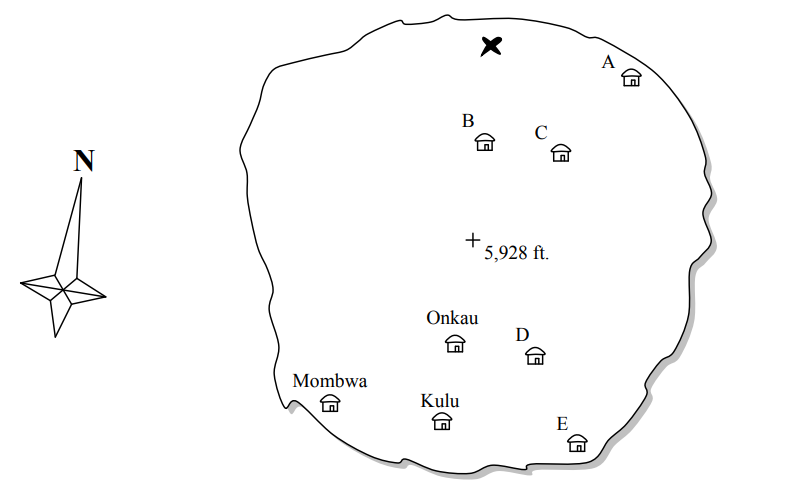
\includegraphics[width = \linewidth]{images/Manam.png}

\begin{assgts}
\item Onkau's, Mombwa's and Kulu's houses have already been located on the map above. Who lives in the other five houses (A-E)?
\item Arongo is building his new house in the location marked with an X on the map. In three Manam Pile sentences like the ones on the previous page, describe the location of Arongo's house in relation to the three closest houses (A-C).
\end{assgts}
\end{problem}

\begin{mysolution}

The first step is identifying the structure of the sentences. This is:

\exrule{\cmubdata{H\textsubscript{1} pera kana X\textsubscript{1} ieno, H\textsubscript{2} pera kana X\textsubscript{2} ieno.}}
 \noindent where H\textsubscript{1} and H\textsubscript{2} refer to the names of the houses. Therefore, X\textsubscript{1} and X\textsubscript{2} must represent the words for directions. We notice that these can be: \cmubdata{ata}, \cmubdata{auta}, \cmubdata{awa}, \cmubdata{ilau}. Moreover, based on the examples 7 and 8, we notice that they can also combine with one another: \cmubdata{ata ilau}, \cmubdata{awa auta}, \cmubdata{awa ilau}, \cmubdata{ata auta}. Therefore, we deduce that there are two main directions or axes: \cmubdata{ata--awa} and \cmubdata{ilau--auta}, which can combine together (similarly to how the directions north--south and east--west can combine to form directions like north-east, north-west, etc.). Furthermore, we notice that X\textsubscript{1} is always the opposite of X\textsubscript{2} (similar to the English sentences \texttr{A is due east, and B due west} or \texttr{A is north-east, and B south-west}).

 Based on this information, we can rewrite the eight sentences above in a simpler way:
     \begin{enumerate}[leftmargin = 5 em]

         \item \texttr{Onkau is to the} \cmubdata{auta} \texttr{of Kulu.}
         \item \texttr{Mombwa is to the} \cmubdata{ata} \texttr{of Kulu.}
         \item \texttr{Tola is to the} \cmubdata{auta} \texttr{of Sala.}
         \item \texttr{Sulung is to the} \cmubdata{awa} \texttr{of Tola.}
         \item \texttr{Sala is to the} \cmubdata{awa} \texttr{of Mombwa.}
         \item \texttr{Pita is to the} \cmubdata{ilau} \texttr{of Sulung.}
         \item \texttr{Sala is to the} \cmubdata{awa ilau} \texttr{of Onkau.}
         \item \texttr{Butokang is to the} \cmubdata{awa auta} \texttr{of Pita.}
     \end{enumerate}

The first hypothesis that comes to mind is that indeed, \cmubdata{ata}, \cmubdata{awa}, \cmubdata{ilau}, and \cmubdata{auta} represent the \texttr{north}, \texttr{south}, \texttr{east}, and \texttr{west}. Thus, based on sentence 1, we deduce that \cmubdata{auta} = \texttr{north}, and based on 2 we deduce that \wordtrans{ata}{west}. Moreover, knowing already that the two main directions are \cmubdata{ata – awa} and \cmubdata{ilau – auta}, we can also deduce the other two cardinal points, mainly \wordtrans{awa}{east} and \wordtrans{ilau}{south}.

Thus, from sentence 7, we find out that Sala's house is to the south-east of Onkau's, so Sala's house can only be E, which is also confirmed by sentence 5, which mentions that Sala's house is to the east of Mombwa's. Next, from sentence 3, we deduce that Tola's house is to the north of Sala's, so Tola's house can only be A or C, but, since sentence 4 says that Sulang's house is to the east of Tola's, Tola's house needs to be C and Sulung's A (if Tola's house were A, there is no other house to the east of it). From sentence 6, Pita's house is to the south of Sulung's, so it is most likely D. Finally, according to sentence 8, Butokang's house is to the north-east of Pita's, but, at the same time, we know that Butokang's house must be B, since it is the only house left. Thus, we reach a contradiction which points to the fact that, most likely, the four words are not cardinal points.

If we carefully read the introduction, we learn that the island is in fact a volcano. Taking this into account, we can interpret the first sentence to mean that Onkau's house is \textit{higher} up the mountain than Kulu's. Since we excluded the possibility that this word (\cmubdata{auta}) means \texttr{north}, perhaps it means \texttr{towards the top} or \texttr{further away from the shore}. Thus, its pair \cmubdata{ilau} will mean \texttr{towards the shore}. We can conclude that the first directional axis is based on altitude (from the sea towards the top of the volcano).

From sentence 2, we understand that we need to find one more direction which points laterally on the map  and we already figured out that it cannot be \texttr{east} and \texttr{west}. Thus, perhaps the words actually represent \texttr{left} and \texttr{right}, when looking towards the top of the volcano. In other words, we can imagine the island to be a clock whose centre is the top of the volcano and the relative positions of the houses are not described by means of east--west but rather clockwise--anticlockwise. Thus, from sentence 2 we deduce that \wordtrans{ata}{clockwise} (\texttr{to the left, facing the volcano}) and, consequently, \wordtrans{awa}{anticlockwise} (\texttr{to the right, facing the volcano}).

Consequently, in sentence 7 we are told that Sala's house is towards the shore and to the right of Onkau's house, so, again, Sala's house can only correspond to E (since D is approximately at the same altitude with Onkau's, so it is not towards the shore). This is also confirmed by sentence 5 which states that Sala's house is anticlockwise with respect to Mombwa's (nothing about the relative vertical position is mentioned, so it is on the same level).

From sentence 3, Tola's house is higher than Sala's, so Tola's house = D. Next, from sentence 4, Sulung's house is anticlockwise of Tola's (to the right, facing the volcano), so Sulung's house = C; from sentence 6, Pita's house is lower than Sulung's (towards the shore), so Pita's house = A. Finally, we are left with B which must be Butokang's house, as confirmed by sentence 8, which states that Butokang's house is higher and to the right of Pita's.

Now we can solve task (b). The house marked with X will be \texttr{towards the shore} with respect to B, \texttr{to the right} of A and \texttr{towards the shore and to the right} of C.

Therefore, we can solve all tasks.

\begin{solutions}
    \item A = Pita, B = Butokang, C = Sulung, D = Tola, E = Sala
    \item \cmubdata{Arongo pera kana awa ieno, Pita pera kana ata ieno.}\\
    \cmubdata{Arongo pera kana awa ilau ieno, Sulung pera kana ata auta ieno.}\\
    \cmubdata{Arongo pera kana ilau ieno, Butokang pera kana auta ieno.}
\end{solutions}
\end{mysolution}

As previously mentioned, with this type of problem, we need to pay attention to the topography of the area and consider the landforms around and how they can be used to indicate directions. In this case, since the language is spoken on an island, it is very plausible that the sea is one of the points of reference. Thus, each point can be closer to the sea or more towards the centre of the island (in this case the middle of the island is actually a volcano so equivalent directions can also be uphill and downhill). Since in the introduction we are told that the island has an active volcano, we expect it to be relevant in solving the problem. Considering that a volcano can be assimilated to a cone, we can consider the second direction to be circular (clockwise or anticlockwise).

\section{Kinship problems}

The core purpose of this type of problem is that different languages use different types of terms to refer to different family relations. This type of problem is very easy to recognise since it will refer to a family tree. In the corpus, some sentences are given in which the relations of some family members with other members of the family are described in the target language.

There are six main types of kinship systems, but before discussing them, it is important to get acquainted with the ways of representing a kinship diagram (a family tree). Figure \ref{fig:short-kinship} shows a basic kinship diagram. Triangles represent men and circles represent women. A double line (an equals sign, =) denotes marriage and simple lines represent blood relations. Figure \ref{fig:short-kinship} tells us that 1 and 3 are two women (they are represented by circles) who are sisters (marked by a simple line), and each of them is married (1 married to 2 and 3 to 4). The family formed by 1 and 2 has two children (vertical line) – a girl (5) and a boy (6), just like the family formed by 3 and 4. Thus, based on this diagram, we can characterise each person with respect to the other, e.g., 6 is the son of 1 and the nephew of 4, 2 is the husband of 1 and the brother-in-law of 3, etc. Generally, linguistics problems will also include a legend which explains the meaning of each symbol, but the notations mentioned above are the standard ones. Moreover, from case to case, some problems might also include the age of the person, since some languages differentiate certain kinship terms based on age (e.g., in Chinese there are different words for \texttr{younger sister} – {\chinesetext{妹妹}} \cmubdata{mèimei}, \texttr{older sister} – {\chinesetext{姐姐}} \cmubdata{jiějie}, \texttr{younger brother} – {\chinesetext{弟弟}} \cmubdata{dìdi}, and \texttr{older brother} – {\chinesetext{哥哥}} \cmubdata{gēge}).

\begin{figure}[h]
  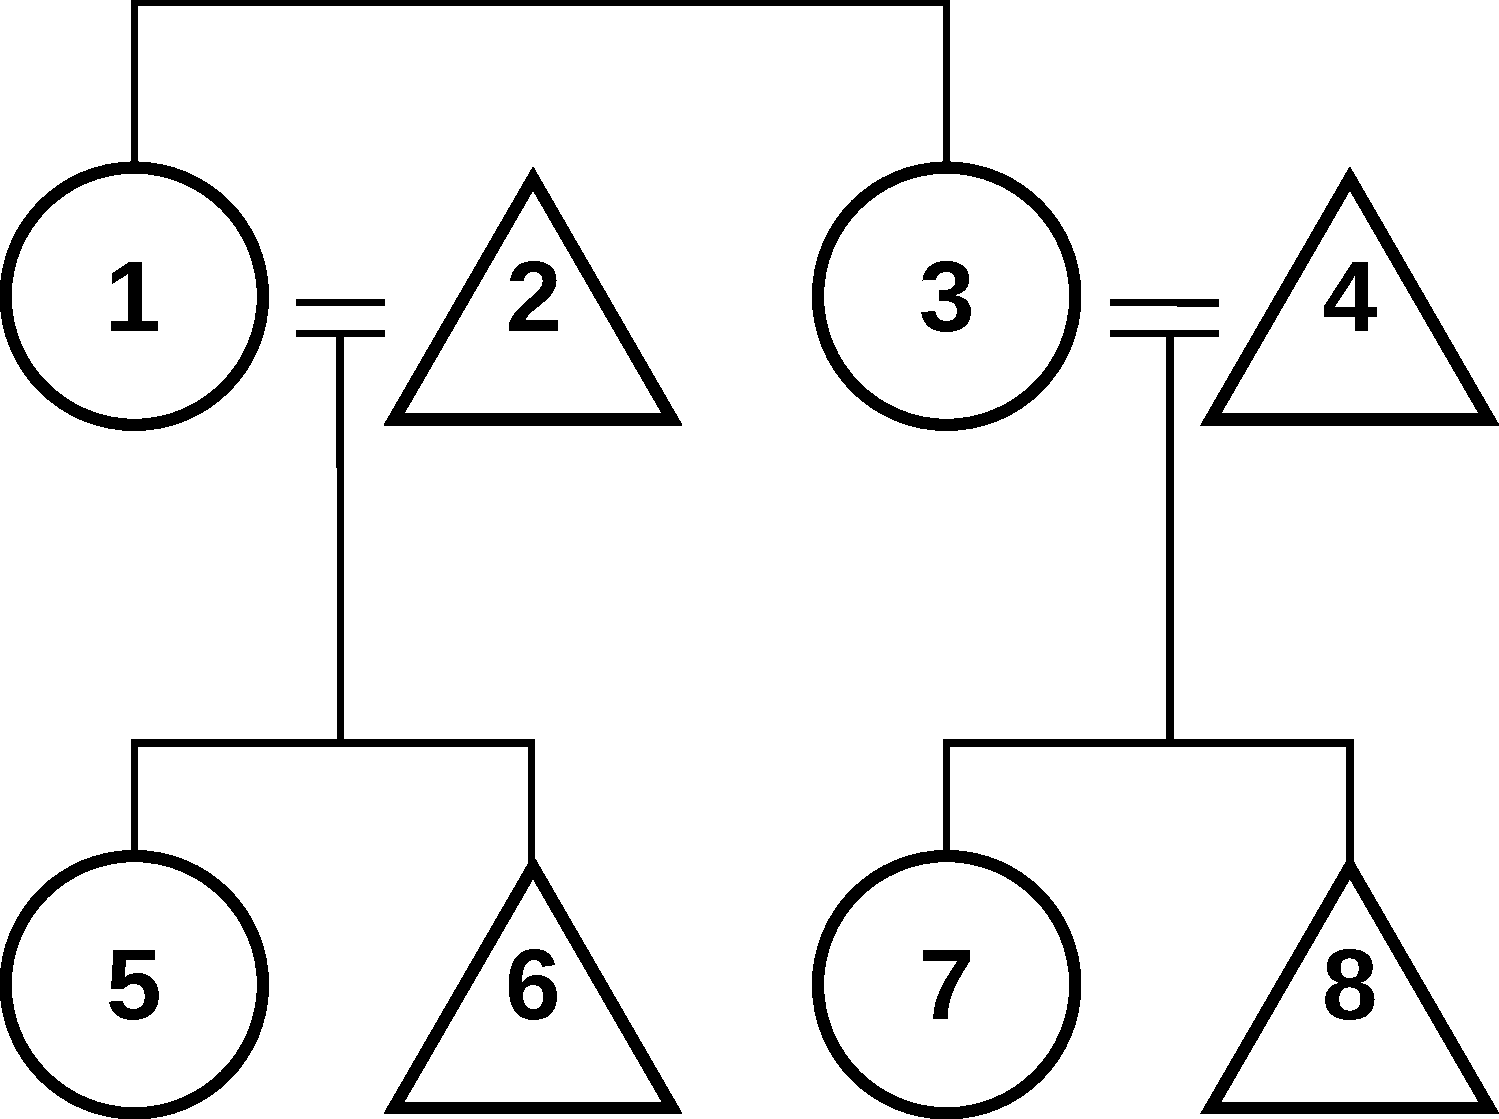
\includegraphics[width = 0.5\linewidth]{figures/kinship_short.pdf}
  \caption{A typical kinship diagram.}
  \label{fig:short-kinship}
\end{figure}

In 1949 the anthropologist G.P. Murdock identified six basic patterns of kinship terminology systems, which are now generally accepted. Of course, certain languages can display systems different from them, but the six types below are the most common ones. 

In order to represent these systems, a diagram like the one in Figure \ref{fig:template-kinship} is used. A shaded triangle or circle, if included, represents the person from whose point of view the tree is presented, called the \textit{Ego} in genealogy.

\begin{figure}[h]
  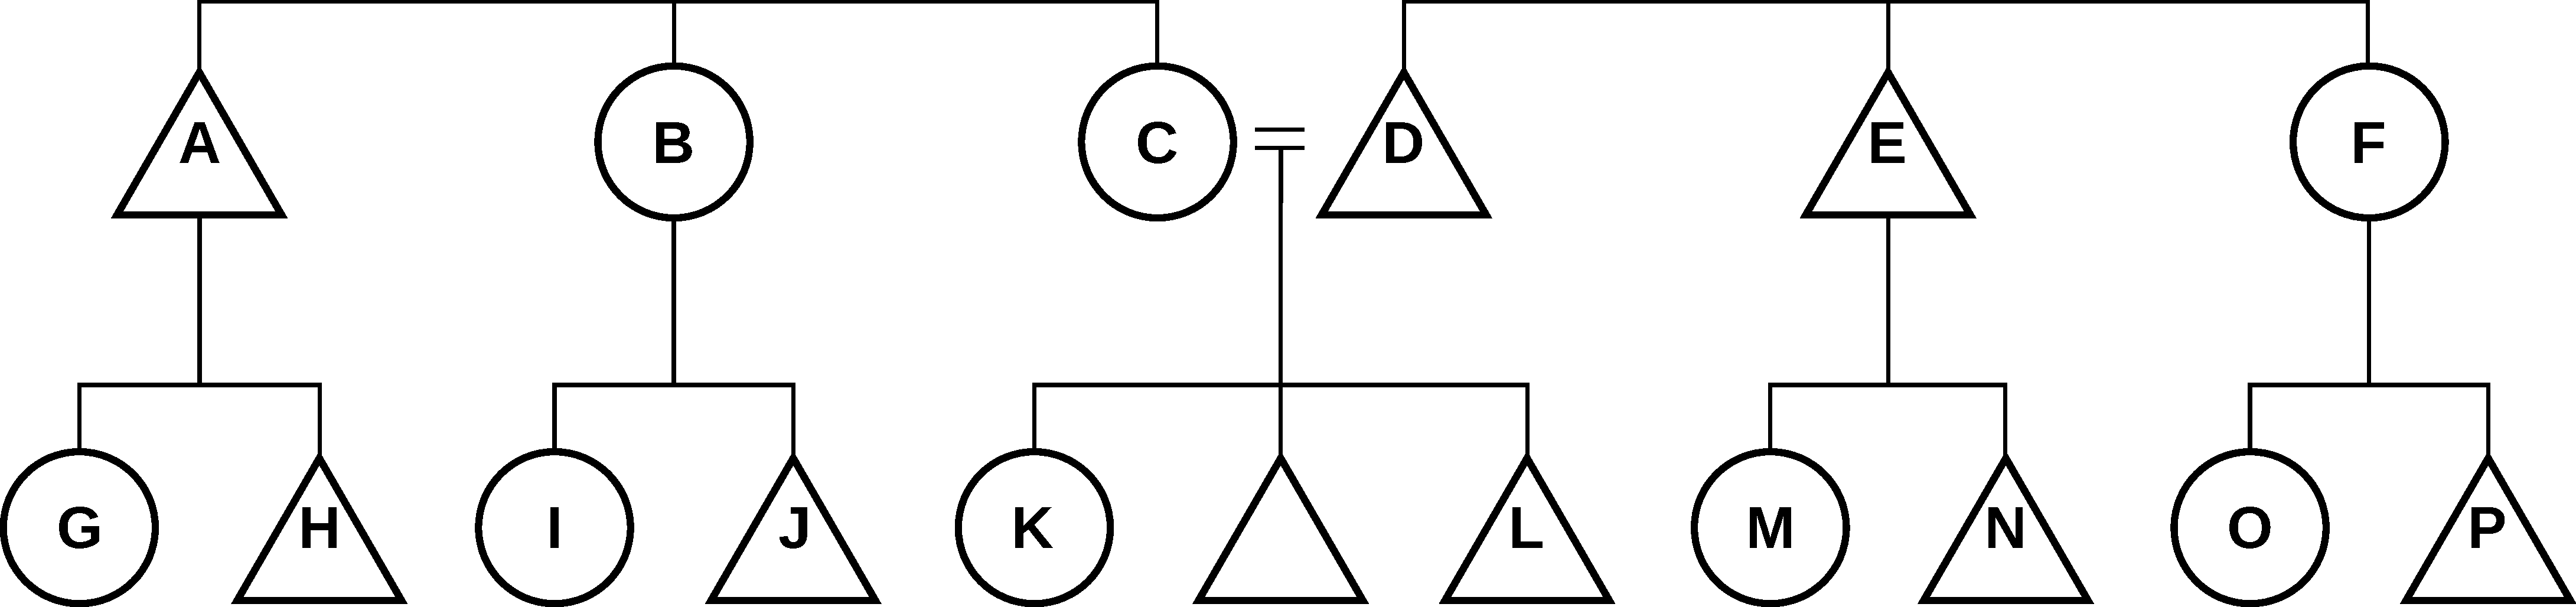
\includegraphics[width = \linewidth]{figures/kinship_template.pdf}
  \caption{Template kinship diagram for describing the different types of kinship systems.}
  \label{fig:template-kinship}
\end{figure}

The simplest kinship system is called \emph{Hawaiian}, which has only three basic kinship terms: \texttr{mother}, \texttr{father} and \texttr{sibling}. Thus, persons A, D and E are all called \texttr{father}, persons B, C, F are all called \texttr{mother} and all siblings and cousins are called the same (\texttr{sibling}). In this case (the Hawaiian system), we write A = D = E, B = C = F and G = H = I = J = K = L = M = N = O = P. This representation does not take into account the variations based on age so, solely based on this description, we cannot know that in the Hawaiian language (which displays the Hawaiian kinship term) there is a difference between younger and older sibling. Generally, in linguistics problems, if the age does not play a relevant role, it will not be included in the diagram (i.e., if a diagram includes the age of the persons, age will certainly play a role).

The next system is called \emph{Eskimo}\footnote{The term dates from 1949 and is still used even though the word \textit{Eskimo} is now disdained as being derogatory.} kinship (or \emph{Inuit}) one, which is also the system used in English. In this system we differentiate C (\texttr{mother}), D (\texttr{father}), B = F (\texttr{aunt}), A = E (\texttr{uncle}), K = L (\texttr{siblings}) and G = H = I = J = M = N = O = P (\texttr{cousins}). Although the six main kinship systems we describe here represent general patterns, these patterns can be slightly modified from one language to another. A case worth mentioning is that of Romanian which, although it is considered to use an Eskimo kinship term, it has two different words for \texttr{cousin} based on the gender, and differentiates between G = I = M = O (\cmubdata{verișoară}, \texttr{female cousin}) and H = J = N = P (\cmubdata{verișor}, \texttr{male cousin}). This is true of many European languages, and in some (e.g. German) the difference \cmubdata{Kusine}--\cmubdata{Vetter} is not just a gender suffix. 

The next system we talk about is called \emph{Sudanese} kinship, one example of which is Turkish, which we use here to illustrate. In this type of system there is a separate term for each of the persons A-F (\wordtrans{dayı}{mother's brother}, \wordtrans{amca}{father's brother}, \wordtrans{teyze}{mother's sister}, \wordtrans{hala}{father's sister}, \wordtrans{anne}{mother}, \wordtrans{baba}{father}) and a different term for each pair of cousins: I and J are called \texttr{maternal parallel cousins} – \textit{maternal} refers to the fact that they are on the mother's side. The term \textit{parallel} is used because the blood relation is from the same-sex persons (i.e., same-sex siblings) - mother and mother's sister (two women). In the same way, O and P are called \texttr{paternal parallel cousins}, from the father's side and, more exactly, from the father's brother (parallel since it is the father's brother (same sex as the father), not sister). The other two categories are called \texttr{maternal cross cousins} and \texttr{paternal cross cousins}, where \textit{cross} refers to the fact that the blood relation is of opposite-sex persons (mother's brother and father's sister).

This distinction between \textit{parallel} and \textit{cross} cousins is rather common and so relevant that in the next kinship system, called \emph{Iroquois} kinship, B = C (\texttr{mother}) and D = E (\texttr{father}). Here, the same-sex siblings of the parents (i.e., mother's sister and father's brother) are also considered to be `parents'. On the other hand, the opposite-sex siblings of the parents are those called \texttr{uncle} (A) and \texttr{aunt} (F). For this reason, G = H = O = P (\texttr{cousins}) -- since they are the children of the aunt and uncle --, but I = J = K = L = M = N (\texttr{siblings}) – since they are the children of the mother and father. The next two systems are derived from this system.

\begin{sloppypar}
The \emph{Crow} kinship system starts from the Iroquois system, with the only change occurring for the persons O and P (the children of the father's sister). They are called \texttr{aunt} (if it is a girl, so O) or \texttr{father} (P). Thus, in this system, D = E = P (\texttr{father}) and F = O (\texttr{aunt}). The rest of the persons follow the Iroquois system (A = \texttr{uncle}, B = C = \texttr{mother}, G = H = \texttr{cousins}, I = J = K = L = M = N = \texttr{siblings}).
\end{sloppypar}

The last system, called \emph{Omaha} kinship, is the opposite of Crow kinship. In this system, a special role is reserved for the children of the mother's brother (instead of father's sister, as in the Crow system). Like the Crow system, the same-sex child is also called \texttr{uncle} or \texttr{aunt}, depending on their (and Ego's) sex (same sex as Ego), while the opposite-sex child is called \texttr{mother} or \texttr{father}. Therefore, A = H = \texttr{uncle}, B = C = G = \texttr{mother}, D = E = \texttr{father}, F = \texttr{aunt}, I = J = K = L = M = N = \texttr{sibling} and O = P = \texttr{cousins}.

Although the systems are each named after a language, there are other languages which follow each system: for example English has `Eskimo kinship', Bulgarian has `Sudanese kinship'.

A comparative representation of these six types of system is represented below:

\vfill
\noindent
{\small\begin{tabular}{|c|c|c|c|c|c|c|}
\hline
Person & {Hawaiian} & {Eskimo} & {Sudanese} & {Iroquois} & {Crow} & {Omaha} \\ \hline
A & \texttr{father} & \texttr{uncle} & \texttr{mother's brother} & \multicolumn{3}{c|}{\texttr{uncle}}  \\ \hline
B & \multirow{2}{*}{\texttr{mother}} & \texttr{aunt} & \texttr{mother's sister} & \multicolumn{3}{c|}{\multirow{2}{*}{\texttr{mother}}}  \\ \cline{1-1} \cline{3-4}
C &  & \multicolumn{2}{c|}{\texttr{mother}} & \multicolumn{3}{c|}{}  \\ \hline
D & \multirow{2}{*}{\texttr{father}} & \multicolumn{2}{c|}{\texttr{father}} & \multicolumn{3}{c|}{\multirow{2}{*}{\texttr{father}}} \\ \cline{1-1} \cline{3-4}
E &  & \texttr{uncle} & \texttr{father's brother} & \multicolumn{3}{c|}{}  \\ \hline
F & \texttr{mother} & \texttr{aunt} & \texttr{father's sister} & \multicolumn{3}{c|}{\texttr{aunt}} \\ \hline
\end{tabular}
\vfill\pagebreak
\noindent
\begin{tabular}{|c|c|c|c|c|c|c|}
\hline
Person & {Hawaiian} & {Eskimo} & {Sudanese} & {Iroquois} & {Crow} & {Omaha} \\ \hline
G & \multirow{10}{*}{\texttr{sibling}} & \multirow{4}{*}{\texttr{cousin}} & \multirow{2}{*}{\texttr{maternal CC}\footnotemark{}} & \multicolumn{2}{c|}{\multirow{2}{*}{\texttr{cousin}}} & \texttr{mother} \\ \cline{1-1} \cline{7-7} 
H &  &  &  & \multicolumn{2}{c|}{} &  \texttr{uncle} \\ \cline{1-1} \cline{4-7} 
I &  &  & \multirow{2}{*}{\texttr{maternal PC}\footnotemark[\value{footnote}]} & \multicolumn{3}{c|}{\multirow{6}{*}{\texttr{sibling}}} \\ \cline{1-1}
J &  &  &  &  \multicolumn{3}{c|}{} \\ \cline{1-1} \cline{3-4}
K &  & \multicolumn{2}{c|}{\multirow{2}{*}{\texttr{sibling}}}  &  \multicolumn{3}{c|}{} \\ \cline{1-1}
L &  &  \multicolumn{2}{c|}{}  &  \multicolumn{3}{c|}{} \\ \cline{1-1} \cline{3-4}
M &  & \multirow{4}{*}{\texttr{cousin}} & \multirow{2}{*}{\texttr{paternal PC}\footnotemark[\value{footnote}]} &  \multicolumn{3}{c|}{} \\ \cline{1-1}
N &  &  &  &  \multicolumn{3}{c|}{} \\ \cline{1-1} \cline{4-7} 
O &  &  & \multirow{2}{*}{\texttr{paternal CC}\footnotemark[\value{footnote}]} & \multirow{2}{*}{\texttr{cousin}} & \texttr{aunt} & \multirow{2}{*}{\texttr{cousin}} \\ \cline{1-1} \cline{6-6}
P &  &  &  &  & \texttr{father} & \\ \hline
\end{tabular}}
\footnotetext{CC = \texttr{cross cousin}, PC = \texttr{parallel cousin}.}

\begin{problem}{\langnameArawak}{\nameMBoron}{\wordoriginal}
Below you can find part of an Arawak family tree. Three family members – two men and a woman (not necessarily in this order) – describe their family:
\begin{enumerate}\sloppy
    \item \cmubdata{De to Fatan. Onikhan to dajo. Mithakotoan ken Kolhen to dakhithonon. Tholhady to dato. Ematonoa to dathi.}
    \item \cmubdata{De to Sobole. Bokoa to dakhithi. Kolhen ken Moty to dajonon. Balhose ken Konoko to dathinon. Onikhan ken Ylhydaba to dakythynon. Fatan ken Mithakotoan to dajaboathonon. Sareke to dajorodatho. Ematonoa to dadokothi.}
    \item \cmubdata{De to Balhose. Ylhydaba to dajo. Kolhen to daretho. Sobole ken Bokoa to daithinon. Konoko to dakhithi. Moty to dajorodatho. Mithakotoan ken Fatan to darebiathonon. Sareke to dato.}
\end{enumerate}
\largerpage[2]
% \noindent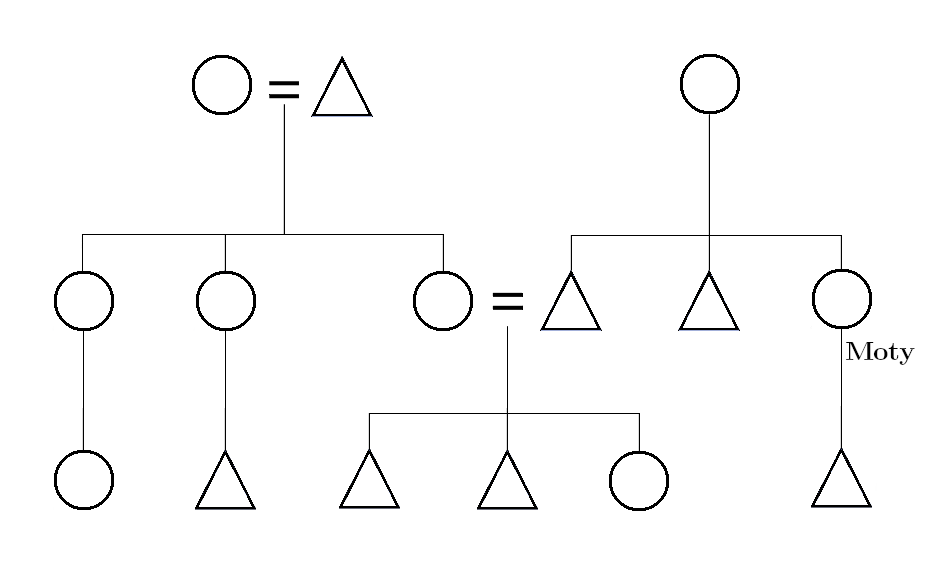
\includegraphics[width = \linewidth]{images/Arawak.png}

\begin{figure}[H]
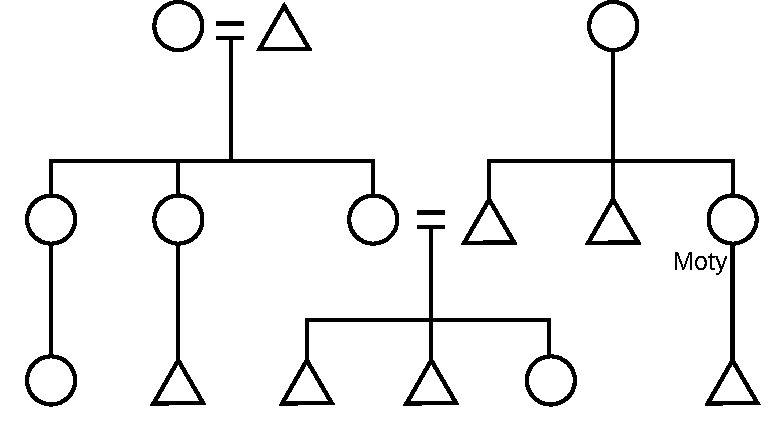
\includegraphics[width = 0.66\linewidth]{figures/Arawak.pdf}
\end{figure}

\begin{assgts}
\item Supply the tree with names. If multiple options are possible, provide them all. 
\item Three more people (from the same family) describe their family:
\begin{enumerate}[start = 4]\sloppy
    \item \cmubdata{De to Ajonym. Fatan ken Kolhen to \pbblank. Onikhan to dakythy. Mithakotoan to dajo. \pbblank to dadokothi.}
    \item \cmubdata{De to \pbblank. Balhose ken Konoko to daithinon. Holholho ken Sobole ken \pbblank  to dalykynthinon. Moty to dato. \pbblank to dalykyntho.}
    \item \cmubdata{De to Kolhen. \pbblank to dajo. \pbblank to darethi. Ematonoa to \\ \pbblank. Sareke to dato. Sobole ken Bokoa to \pbblank. Konoko to \pbblank.}
\end{enumerate}
\item[] Fill each gap with \textit{exactly one word}. 
\end{assgts}

\begin{tblsWarning}
In the diagram above, triangles represent men and circles represent women. Horizontal lines represent siblings and vertical lines children. The equals sign denotes marriage. 
\end{tblsWarning}
\end{problem}

\begin{mysolution}

Firstly, we look at the structure of the sentences. Each sentence, except for the first, follows the pattern Name \cmubdata{to} X. So we know that X represents the kinship term. We deduce that \wordtrans{ko}{is/are}, and the first sentence most likely means \texttr{I am X}, therefore \wordtrans{de}{I}. Moreover, we notice that if in the rest of the sentences there are more names co-occurring, they are separated by \cmubdata{ken}, so this word most likely means \texttr{and}. Last but not least, we notice that every time that a sentence contains more than one name, the kinship term ends in \cmubdata{non}, so we deduce that the suffix \cmubdata{-non} marks the plural.

Based on this we can make a table in which we show the relations between the persons mentioned in the data:

\begin{longtable}{llll}
\lsptoprule
      & Fatan & Sobole & Balhose \\ \midrule\endfirsthead
\midrule
      & Fatan & Sobole & Balhose \\ \midrule\endhead
Fatan & \cellcolor[HTML]{808080} & \cmubdata{dajaboatho} & \cmubdata{darebiatho} \\ 
Onikhan & \cmubdata{dajo} & \cmubdata{dakythy} &  \\ 
Mithakotoan & \cmubdata{dakhitho} & \cmubdata{dajaboatho} & \cmubdata{darebiatho} \\ 
Kolhen & \cmubdata{dakhitho} & \cmubdata{dajo} & \cmubdata{daretho} \\ 
Tholhady & \cmubdata{dato} &  &  \\ 
Ematonoa & \cmubdata{dathi} & \cmubdata{dadokothi} &  \\ 
Sobole &  & \cellcolor[HTML]{808080} & \cmubdata{daithi} \\ 
Bokoa &  & \cmubdata{dakhithi} & \cmubdata{daithi} \\ 
Moty &  & \cmubdata{dajo} & \cmubdata{dajorodatho} \\ 
Balhose &  & \cmubdata{dathi} & \cellcolor[HTML]{808080} \\ 
Konoko &  & \cmubdata{dathi} & \cmubdata{dakhithi} \\ 
Ylhydaba &  & \cmubdata{dakythy} & \cmubdata{dajo} \\ 
Sareke &  & \cmubdata{dajorodatho} & \cmubdata{dato} \\ 
\lspbottomrule
\end{longtable}

Moreover, we notice that two names are missing: \emph{Ajonym} and \emph{Holholho} (both of them found in task (b)).

Generally, the first step in solving this type of problem, once the table above is made, is assuming that if two persons have the same relation with a third, then those two persons belong to the same generation (e.g., if A and B are \emph{m} to person X -- or X is \emph{m} to persons A and B -- then, most likely, A and B are part of the same generation, i.e., they are on the same level of the tree). In this case, we notice from the diagram that we have three generations: the top one, which has three members, the middle one (siz members) and the bottom one (six members).

Starting with Fatan, we notice that they are the same relation (\cmubdata{dakhitho}) to both Mithakotoan and Kolhen, so we can assume that these two belong to the same generation. Similarly, we deduce that Fatan and Mithakotoan belong to the same generation (since they both are \cmubdata{dajaboatho} to Sobole). Knowing that Mithakotoan and Kolhen as well as Mithakotoan and Fatan belong to the same generation, we can deduce that all three of them are part of the same generation.

Using the same thought process, we get the following pairs of persons belonging to the same generation: Kolhen – Moty (they are \cmubdata{dajo} for Sobole), Balhose – Konoko (\cmubdata{dathi} for Sobole), Fatan – Mithakotoan (\cmubdata{darebiatho} for Balhose), Sobole – Bokoa (\cmubdata{daithi} for Balhose), Onikhan – Ylhydaba (\cmubdata{dakythy} for Sobole).

Collecting all the information, we get: 

\begin{description}[font=\normalfont]
\item[Group 1:] Mithakotoan – Kolhen – Fatan – Moty
\item[Group 2:] Balhose – Konoko
\item[Group 3:] Sobole – Bokoa
\item[Group 4:] Onikhan – Ylhydaba
\end{description}

We need to take into account that two (or more) of these groups can combine to form a generation. Moreover, we know for sure that Group 1 is part of the middle generation since it contains Moty.

Furthermore, we can use task (b) to see if there are any other names that cooccur. In example 5, sentence 3, we notice that Holholho and Sobole appear together. At first sight, it can seem insignificant since we have no information about Holholho in the corpus. However this information is actually extremely important. If we add Holholho to Group 3, then this group will contain three persons. Since Group 1 has four persons and Group 3 has three persons, we certainly know that these two cannot represent the same generation (since there is no generation with seven members), so we deduce that Group 1 and Group 3 belong to different generations.

Let us look now at the kinship term \cmubdata{dajo}. It appears between Sobole (Group 3) and Kolhen (Group 1), so we know that this term spans across generations. The same relation appears between Fatan (Group 1) and Onikhan (Group 4). Based on this, we deduce that Group 4 represents the last separate generation (it does not combine with either Group 1 or Group 3). This might not seem obvious at first, but we know that the relation between a person from Group 3 and a person from Group 1 is the same as the relation between a person from Group 1 and one from Group 4 (we can write this succinctly as G3--G1 = G1--G4). Moreover, we already know that G3 and G1 belong to different generations, so, if G4 belonged to the same generation as G1, then the second relation (the word \cmubdata{dajo} which refers to Kolhen from G1 and Onikhan from G4) would be within the same generation, while this is not true for the first relation (the word \cmubdata{dajo} which refers to G3--G1). If G4 was part of the same generation as G3, then we would have a reciprocal relation (the relation of X to Y uses the same name as the relation of Y to X – but across different generations), which is highly unlikely. The only option left is, therefore, that G4 belongs to a separate generation.

Let us focus now on the relation \cmubdata{dajo}, which appears between Onikhan (G4) and Fatan (G1), as well as between Ylhydaba (G4) and Balhose (G2) (i.e., G4--G1 = G4--G2). From here, we deduce that G2 and G1 belong to the same generation.

Now we can classify the three generations:\largerpage[2]

\begin{description}[font=\normalfont]
    \item[Generation A (Gen. A):] Mithakotoan, Kolhen, Fatan, Moty, Balhose, Konoko
    \item[Generation B (Gen. B):] Sobole, Bokoa, Holholho
    \item[Generation C (Gen. C):] Onikhan, Ylhydaba
\end{description}

For simplicity, we can remake the table, but this time replacing the name with the generation.

\begin{table}[H]
\begin{tabular}{ *4{l} }
\lsptoprule
  & A & B & A \\ \midrule
A & \cellcolor[HTML]{808080} & \cmubdata{dajaboatho} & \cmubdata{darebiatho} \\ 
C & \cmubdata{dajo} & \cmubdata{dakythy} &  \\ 
A & \cmubdata{dakhitho} & \cmubdata{dajaboatho} & \cmubdata{darebiatho} \\ 
A & \cmubdata{dakhitho} & \cmubdata{dajo} & \cmubdata{daretho} \\ 
Tholhady & \cmubdata{dato} &  &  \\ 
Ematonoa & \cmubdata{dathi} & \cmubdata{dadokothi} &  \\ 
B &  & \cellcolor[HTML]{808080} & \cmubdata{daithi} \\ 
B &  & \cmubdata{dakhithi} & \cmubdata{daithi} \\ 
A &  & \cmubdata{dajo} & \cmubdata{dajorodatho} \\ 
A &  & \cmubdata{dathi} & \cellcolor[HTML]{808080} \\ 
A &  & \cmubdata{dathi} & \cmubdata{dakhithi} \\ 
C &  & \cmubdata{dakythy} & \cmubdata{dajo} \\ 
Sareke &  & \cmubdata{dajorodatho} & \cmubdata{dato} \\ 
\lspbottomrule
\end{tabular}
\end{table}

The first observation is that both Tholhady and Sareke have the relation \cmubdata{dato} with respect to Gen. A, so they both belong to the same generation (B or C, since Gen. A already has six members, so it is complete).

The term \cmubdata{dajorodatho} is established between two persons from Gen. A, so it is a kind of relation established within the same generation. Since Sareke uses the same relation with a person from Gen. B, we deduce that Sareke also belongs to Gen. B.

For Ematonoa, we look at the term \cmubdata{dathi}. We have the equivalence: A--B = Ematonoa--A. Since we said we exclude transitive relations, Ematonoa must belong to Gen. C. Thus, the generations become:

\begin{description}[font=\normalfont]
    \item[Gen. A:] Mithakotoan, Kolhen, Fatan, Moty, Balhose, Konoko
    \item[Gen. B:] Sobole, Bokoa, Holholho, Tholhady, Sareke
    \item[Gen. C:] Onikhan, Ylhydaba, Ematonoa
\end{description}

There is only one person unassigned, Ajonym, who surely belongs to Gen. B (since it is the only incomplete generation in terms of the number of members). Moreover, we know the correspondence between the letters A--C and the top/middle/bottom generations. Gen. C is surely the top one, since it has only three members, while Gen. A is the middle one since it contains Moty. Therefore, Gen. B remains and must be the bottom one. The final generations are:

\begin{description}[font=\normalfont]
    \item[Top generation:]  Onikhan, Ylhydaba, Ematonoa
    \item[Middle generation:]  Mithakotoan, Kolhen, Fatan, Moty, Balhose, Konoko
    \item[Bottom generation:]  Sobole, Bokoa, Holholho, Tholhady, Sareke, Ajonym
\end{description}

We expect that the kinship terms established between the middle and the top generation to be \texttr{mother} and \texttr{father} (the other option is something like \texttr{wife's sister's mother}, which is rather too complex). Thus, we notice that for Fatan, Onikhan and Ematonoa are \cmubdata{dathi} and \cmubdata{dajo}, respectively; we can assume that they represent \texttr{mother} and \texttr{father}. Since there is only one married couple in the top generation, it must be Onikhan-Ematonoa. To differentiate between \texttr{mother} and \texttr{father}, we notice that \cmubdata{dajo} also appears with Ylhydaba, who belongs to the top generation. Since the only person left in the top generation is a woman, we deduce that \wordtrans{dajo}{mother} and \wordtrans{dathi}{father}. Moreover, we can assign all the names to the top generation (from left to right: Onikhan, Ematonoa, Ylhydaba).

We notice that for Sobole, both Onikhan and Ylhydaba are \cmubdata{dakythy}. Since Sobole is part of the bottom generation, we can easily deduce that \wordtrans{dakythy}{grandmother}. Moreover, we deduce that Sobole must be one of the children in the middle of the tree (the group of three siblings), since they are the only persons whose grandparents are both Onikhan and Ylhydaba.

Let us now look at Sobole's statements. Since we already know the words for \texttr{mother} and \texttr{father}, we notice that in the generation above, Sobole has two persons who they refer to as \cmubdata{dajo} \texttr{mother} (Kolhen and Moty), two who they call \cmubdata{dathi} \texttr{father} (Konoko and Balhose) and two who they refer to as \cmubdata{dajaboatho} (Fatan and Mithakotoan). Among the two persons called \texttr{mother}, we can surely expect that one of them but not both is their biological mother. Since we already know where Moty is placed, we deduce that Kolhen is the (biological) mother of Sobole (the married woman). Moreover, certainly the two men will be those called \texttr{father} (Konoko and Balhose), and the two remaining women on the right will be Fatan and Mithakotoan. Furthermore, the relation between Fatan and Mithakotoan is \cmubdata{dakhitho}, so \wordtrans{dakhitho}{sister (of a woman)}. Similarly, the relation between Konoko and Balhose is \cmubdata{dakhithi}, so \wordtrans{dakhithi}{brother (of a man)}. Next, we notice the similarity between the two terms, which differ only in terms of their last vowel (\cmubdata{-i} or \cmubdata{-o}), which makes us assume that the difference in gender is marked by the last vowel (thus, the stem \cmubdata{dakhith-} means \texttr{same-sex sibling}; if it ends in the vowel \cmubdata{-i}, meaning masculine, it will refer to same-sex brothers i.e., brother of a male, while if it receives the suffix \cmubdata{-o}, it means same-sex sister, i.e., a woman's sister).

We also notice that Bokoa and Sobole are \cmubdata{dakhithi}, so the two are siblings. Therefore, Sobole and Bokoa are the two men from the bottom generation. Moreover, the two men are \cmubdata{daithi} for Balhose, so \wordtrans{daithi}{son}. We can assume that Balhose is the biological father of the two children (unlike Konoko). This is also confirmed by the fact that Kolhen is \cmubdata{daretho} for Balhose, and this kinship term does not occur again, so it means that \wordtrans{daretho}{wife}.

Sareke is \cmubdata{dato} for Balhose, and Sareke is part of the bottom generation. The only person, in relation with Balhose, which we have not described, is their daughter, so Sareke is the daughter of Balhose (the sister of Sobole and Bokoa), and \wordtrans{dato}{daughter}.

Furthermore, since Tholhady is the daughter of Fatan (knowing that Fatan and Mithakotoan are the two women in the middle generation, and only one of them has a daughter), we can determine all the correspondences of the middle generation. The names are, from left to right: Fatan, Mithakotoan, Kolhen, Balhose, Konoko, Moty.

The only persons left to be assigned to the diagram are Ajomyn and Holholho. Checking task (b), sentence 4, Ajonym says that Onikhan is their \cmubdata{dakythy} \texttr{grandmother}, so Ajonym is the son of Mithakotoan, while Holholho is the son of Moty.

The only thing left undetermined is the difference between Sobole and Bokoa. Since we have no information which could help differentiate between the two (and since task (a) says that there are multiple options in some cases), we deduce that the correct assignment of names is as presented in Figure \ref{fig:arawak-solution} (with the mention that Sobole and Bokoa can be swapped).

\vfill
\begin{figure}[H]
  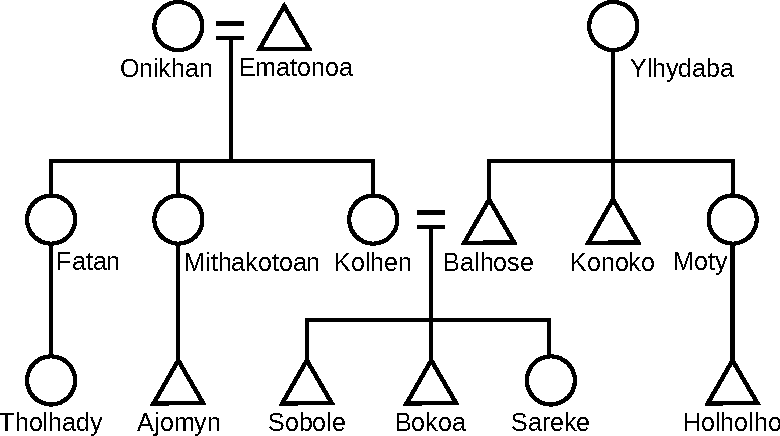
\includegraphics[width = 0.66\linewidth]{figures/Arawak_withNames.pdf}
  \caption{The name assignment for Problem 10.2.}
  \label{fig:arawak-solution}
\end{figure}
\vfill\pagebreak

Based on this, we can easily deduce the remaining kinship terms, and make a table with all the words we know (since we saw that the masculine-feminine pairs are similar, we organise them in different columns):

\begin{table}[H]
    \begin{tabular}{ lll }
    \lsptoprule
    Kinship term & Male & Female \\\midrule
    \texttr{child} & \cmubdata{daithi} & \cmubdata{dato} \\
    \texttr{parent} or \texttr{father's sibling} & \cmubdata{dathi} & \cmubdata{dajo} \\
    \texttr{grandparent} & \cmubdata{dadokothi} & \cmubdata{dakythy} \\
    \texttr{grandchild} & \cmubdata{dalykynthi} & \cmubdata{dalykyntho} \\
    \texttr{same-sex sibling} & \cmubdata{dakhithi} & \cmubdata{dakhitho} \\
    \texttr{opposite-sex sibling} & \cmubdata{} & \cmubdata{dajorodatho} \\
    \texttr{spouse} & \cmubdata{darethi} & \cmubdata{daretho} \\
    \texttr{spouse's same-sex sibling} & \cmubdata{darebiathi} & \cmubdata{darebiatho} \\
    \texttr{mother's sibling} & \cmubdata{} & \cmubdata{dajaboatho} \\
    \lspbottomrule
    \end{tabular}
\end{table}

We notice again that some kinship terms can switch between masculine and feminine by changing the last vowel from \cmubdata{-i} (masculine) to \cmubdata{-o} (feminine).

Based on this, we can solve task (b):
\begin{multicols}{3}
\begin{enumerate}[label = (\arabic*)]
    \item \cmubdata{dajaboathonon}
    \item \cmubdata{Ematonoa}
    \item \cmubdata{Ylhydaba}
    \item \cmubdata{Bokoa}
    \item \cmubdata{Sareke}
    \item \cmubdata{Onikhan}
    \item \cmubdata{Balhose}
    \item \cmubdata{dathi}
    \item \cmubdata{daithinon}
    \item \cmubdata{darebiathi}
\end{enumerate}
\end{multicols}
\end{mysolution}

\hypertarget{practice-problems}{%
\section{Practice problems}}

\begin{problem}{\langnameBardi}{\nameCSheard}{\LOYear{\UKLOAbbr}{2012}}
In the picture below, note that both you and the speaker are facing the paper. The bird is to the left of everything else and the kangaroo is to the right of everything else. The cat is behind everything else and the kangaroo is in front of everything else.

\begin{center}
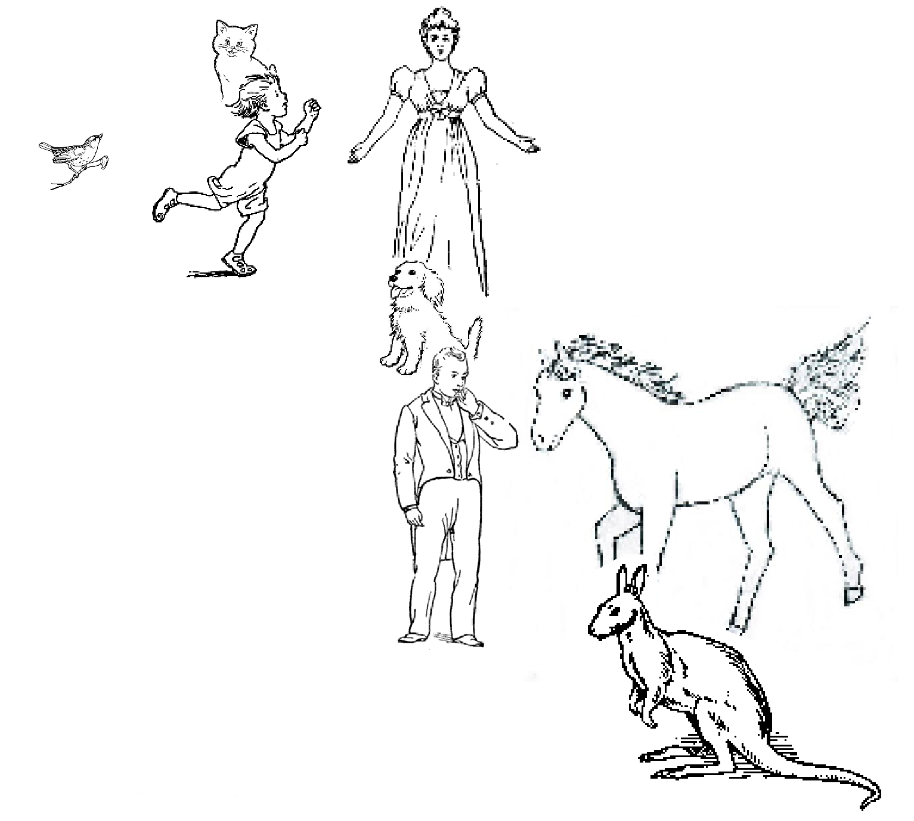
\includegraphics[width = 10 cm]{images/Bardi.png}
\end{center}
Here are some Bardi sentences describing the scene:
\begin{enumerate}[label = \roman*), leftmargin = 1in]
    \item \cmubdata{Aamba bornkony yaawardon.}
    \item \cmubdata{Baawa joorroonggony garrabalgoon.}
    \item \cmubdata{Boorroo alaboor yaawardon.}
    \item \cmubdata{Iila alaboor ooranygoon.}
    \item \cmubdata{Iila baybirrony aambon.}
    \item \cmubdata{Minyaw baybirrony baawon.}
    \item \cmubdata{Oorany joorroonggony baawon.}
    \item \cmubdata{Yaawarda bornkony aambon.}
\end{enumerate}
\pagebreak
\begin{assgts}
\item Based on these, determine the following correspondences:
\begin{center}
    \begin{tabular}{rl@{\hskip0.5in}cl}
         \chaosline{Aarlgoodony}{bird}
         \chaosline{Aamba}{child}
         \chaosline{Alaboor}{cat}
         \chaosline{Baawa}{dog}
         \chaosline{Baybirrony}{horse}
         \chaosline{Boorroo}{kangaroo}
         \chaosline{Bornkony}{man}
         \chaosline{Garrabal}{woman}
         \chaosline{Iila}{next to}
         \chaosline{Joorroonggony}{behind}
         \chaosline{Minyaw}{in front of}
         \chaosline{Oorany}{to the left of}
         \chaosline{Yaawarda}{to the right of}
    \end{tabular}
\end{center}
\end{assgts}
\end{problem}

\begin{problem}{\langnameKharia}{\nameBDohnalova}{\LOYear{\CLOAbbr}{2021}}
Below is shown the kinship tree of a Kharia family in which circles represent women and squares represent men. The age of each person is written under their name.
\vfill
\begin{figure}[H]
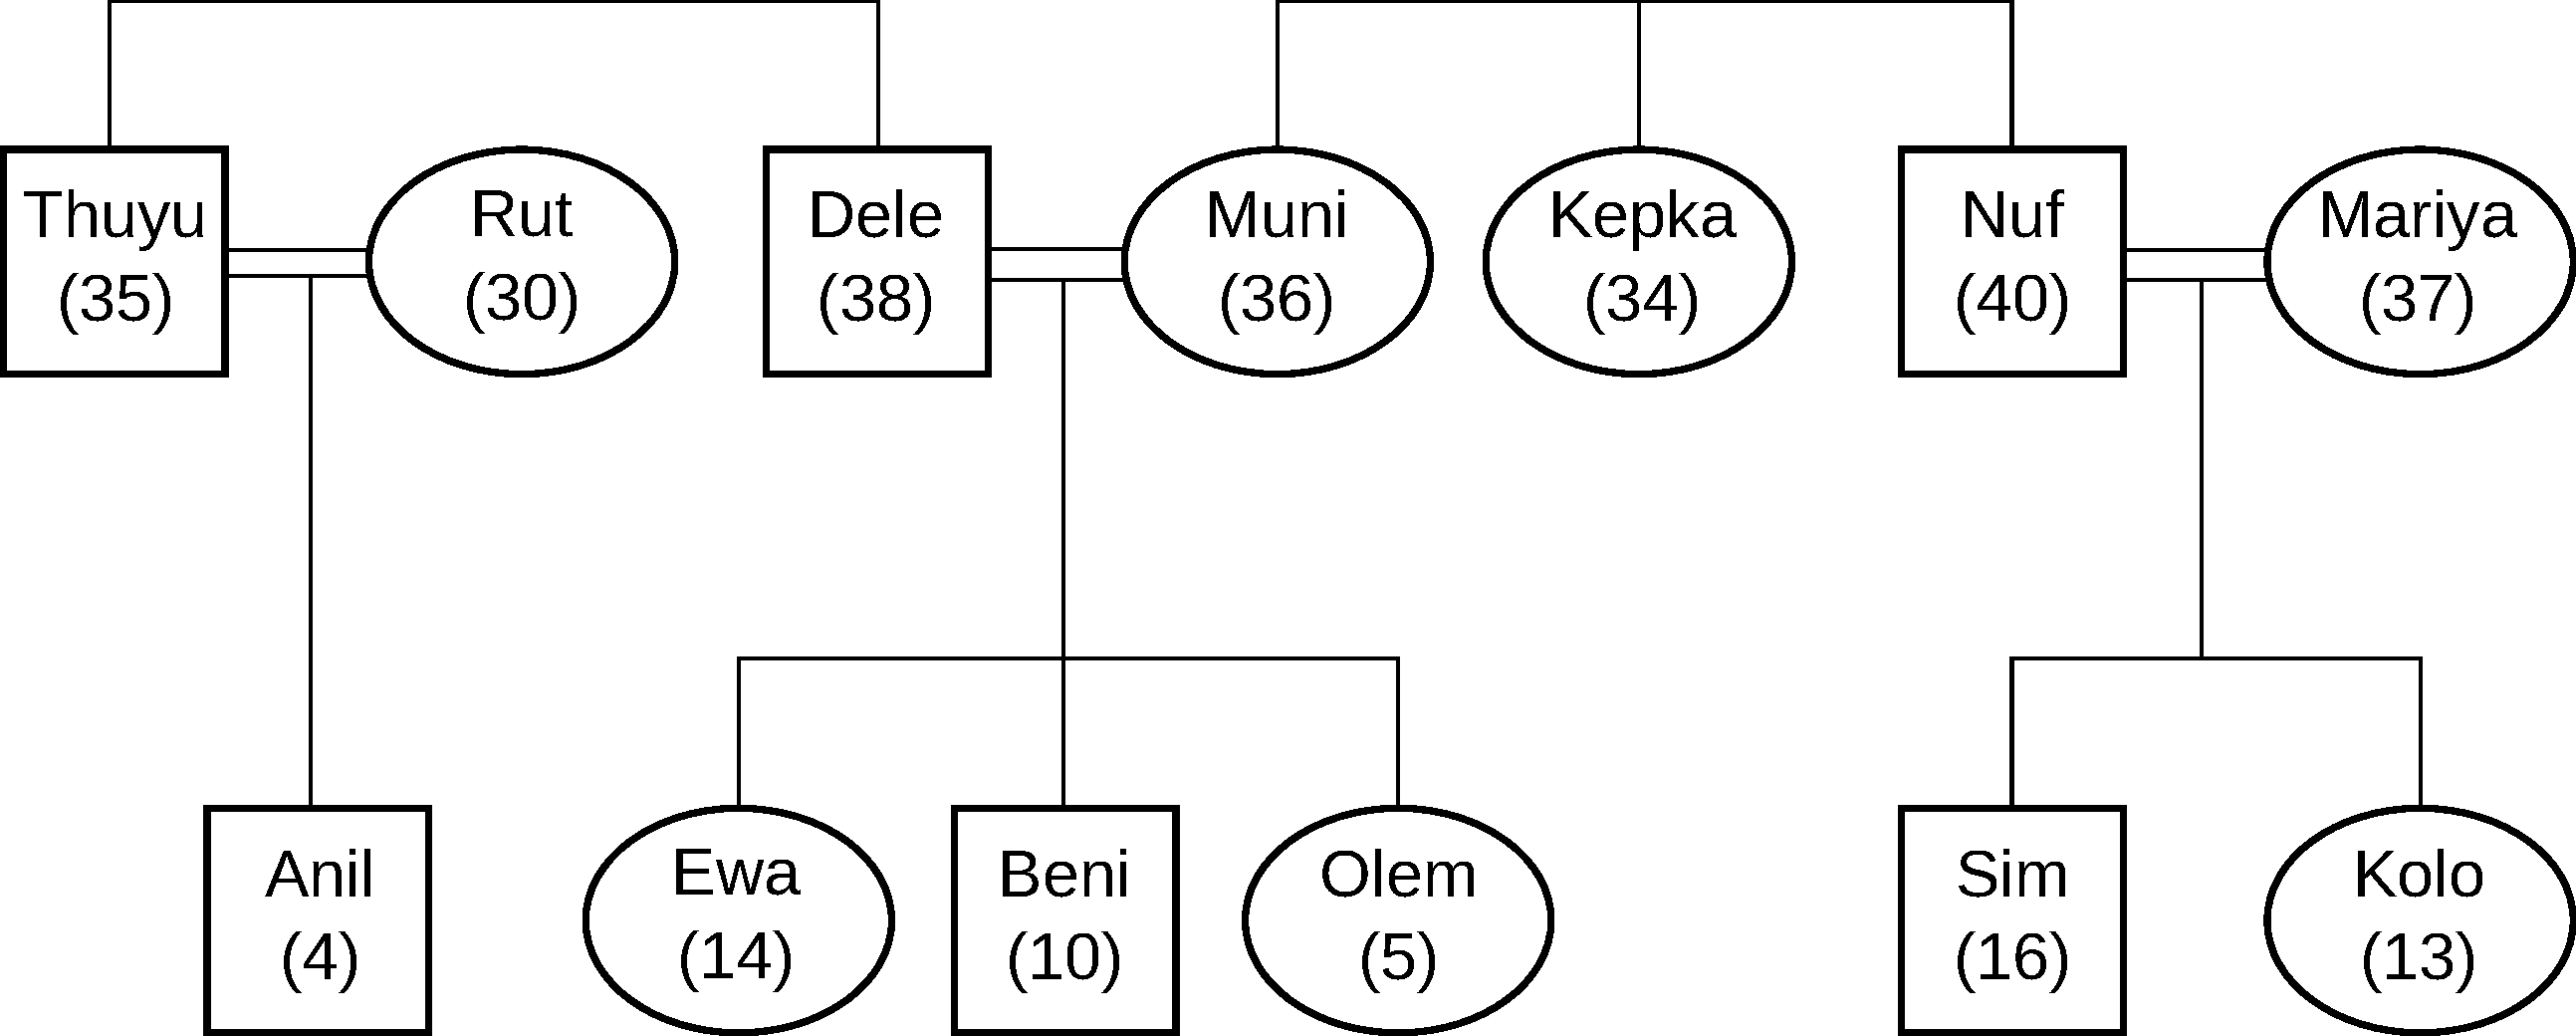
\includegraphics[width = \linewidth]{figures/Kharia.pdf}
\end{figure}
\vfill\pagebreak

Each member of this family says something about their family in Kharia: 
\begin{enumerate}[label = \alph*.]
    \item \cmubdata{Bhaiiɲaʔ ɲimi Thuyu.}
    \item \cmubdata{Didiiɲaʔ ɲimi Muni. Ɖonkuiiɲaʔ ɲimi Mariya.}
    \item \cmubdata{Sowiɲaʔ ɲimi Nuh.}
    \item \cmubdata{Didikiiɲaʔ ɲimiki Olem oɖoyoʔ no Ewa.}
    \item \cmubdata{Konon bahiniɲaʔ ɲimi Olem. Didikiiɲaʔ ɲimiki Ewa oɖoyoɁ no Kolo.}
    \item \cmubdata{Ɖonkuiiɲaʔ ɲimi Muni. Dad=iɲaʔ ɲimi Dele.}
    \item \cmubdata{Sowiɲaʔ ɲimi Thuyu. Be\textsuperscript{ʔ}ʈiɲaʔ ɲimi Anil.}
    \item \cmubdata{Dadakiiɲaʔ ɲimiki Beni oɖoyoʔ no Sim.}
    \item \cmubdata{Be\textsuperscript{ʔ}ʈiɲaʔ ɲimi Beni. Ɖonkuiiɲaʔ ɲimi Mariya.}
    \item \cmubdata{Bhaikiiɲaʔ ɲimiki Beni oɖoyoʔ no Anil. Apaiɲaʔ ɲimi Dele.}
    \item \cmubdata{Konon bahinkiiɲaʔ ɲimiki Kolo, Ewa oɖoyoʔ no Olem.}
    \item \cmubdata{Konon bahinkiiɲaʔ ɲimiki Muni oɖoyoʔ no Kepka.}
    \item \cmubdata{Apaiɲaʔ ɲimi Nuh. Dad=iɲaʔ ɲimi Sim.}
\end{enumerate}
\begin{assgts}
\item Assign each of the sentences above to the person who uttered it.
\item Fill in the blanks:
\begin{enumerate}[label = \roman*.]
    \item Muni: “\cmubdata{\pbblank ɲimi Dele.}”
    \item Kepka: “\cmubdata{\pbblank ɲimi Nuh.}”
    \item Ewa: “\cmubdata{Konon bahinkiiɲaʔ ɲimiki \pbblank.}”
    \item Anil: “\cmubdata{Dad=iɲaʔ ɲimi  \pbblank.}”
    \item Beni: “\cmubdata{\pbblank ɲimi Dele.}”
\end{enumerate}
\item A few years later, Kepka has a son named Caitu. Fill in the blanks:
\begin{enumerate}[label = \roman*., start = 6]
    \item Sim: “\cmubdata{\pbblank ɲimi Caitu.}”
    \item Kepka: “\cmubdata{\pbblank ɲimi Caitu.}”
    \item Caitu: “\cmubdata{\pbblank ɲimiki Ewa, Olem oɖoyoʔ no Kolo.}”
\end{enumerate}
\end{assgts}
\end{problem}

\begin{problem}{\langnameEmbaloh}{\nameKGilyarova}{\LOYear{\MSKAbbr}{2006}}
A tourist travels to a village on the course of the river Benoit Martinus Ambala (Kalimantan Island, Indonesia), in order to learn the Embaloh language. He will live at the Chief's House (see map). On the first day, the Chief takes his guest outside, points towards the north, south, east and west and says “urait, kalaut, anait, suali”. The tourist wrote down in his own dictionary: \wordtrans{urait}{north}, \wordtrans{kalaut}{south}, \wordtrans{anait}{east}, \wordtrans{suali}{west}.\largerpage[2]

\begin{figure}
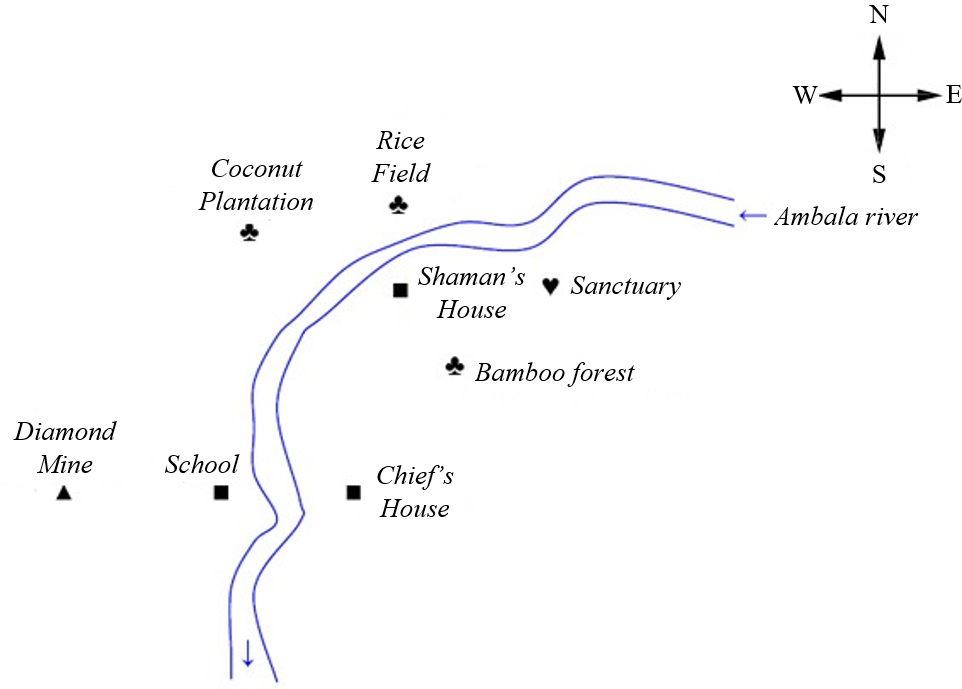
\includegraphics[width = \linewidth]{images/Embolah_EN.png}
\end{figure}

The next day, the tourist wanted to visit the Sanctuary – the place where all the important tribal ceremonies take place. He took his dictionary and compass, but he left his map at home. Exiting the Chief's House, he started walking north and reached the Shaman's House. He asked the Shaman: “How can I get to the Sanctuary?”\ “Keep going \cmubdata{urait},”\ replied the Shaman. “So, I should head north”\ thought the tourist, checking his dictionary. He crossed the river, but then he got lost in a Rice Field, so he decided to return to the Shaman. A plantation worker guided him: “Towards the Shaman's House, go \cmubdata{suali}.” “That means west?! Weird!” thought the tourist, but nevertheless he headed west. However, the river didn't come up and the rice fields were slowly replaced by coconut plantations and the tourist realised he was completely lost. “Whatever it is,”\ a worker on the coconut plantation started comforting the tourist, “keep going \cmubdata{kalaut}. You will get to the School and the teacher will explain everything.”

Checking his dictionary, he headed south and he indeed reached the school. “Chief's House \cmubdata{anait}?”\ the tourist asked the teacher. “No, \cmubdata{anait} Diamond Mine. Chief's House \cmubdata{suali}”\ he replied. The tourist, humbled, headed west and found himself at the Diamond Mine. Extremely angry, he asked: “How can I finally reach the Chief's House or at least the School?”\ “Chief's House \cmubdata{suali}, but School \cmubdata{andoor}.”\ Unfortunately, this last word does not appear in the tourist's dictionary.

\begin{assgts}
\item Explain why the tourist got lost and explain how the orientation system of this tribe works, as well as what each direction means.
\item Describe in Embolah the directions:
\begin{enumerate}
    \item from the Sanctuary to the Shaman's House;
    \item from the Bamboo Forest to the Shaman's House;
    \item from the Shaman's House to the Rice Field.
\end{enumerate}
\end{assgts}
\end{problem}\largerpage[2]

\begin{problem}{\langnameHungarian}{\nameAHesterberg}{\LOYear{\UKLOAbbr}{2014}}
The picture below represents a field divided into 49 squares (7x7), aligned with north at the top and east on the right. In some of the squares there are rocks, indicated by a black circle ●. 

\begin{figure}[H]
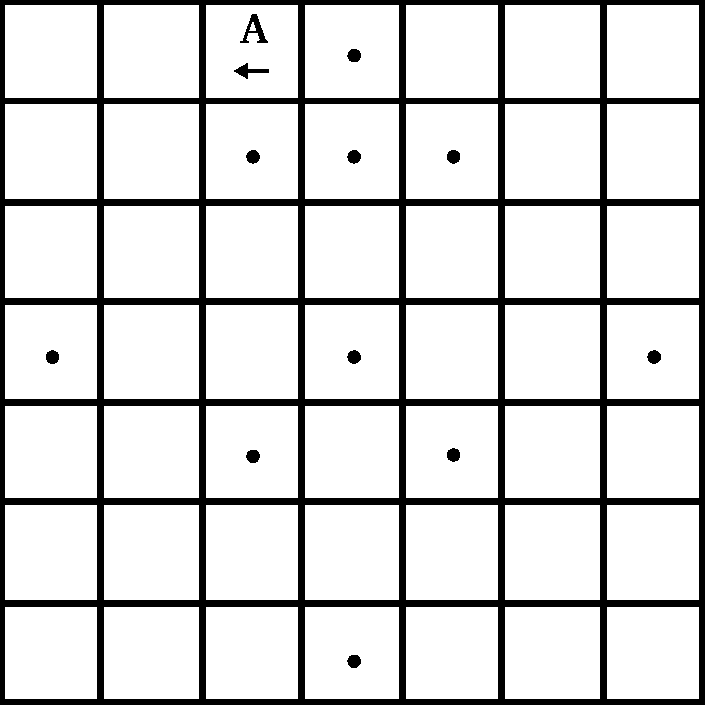
\includegraphics[width = 6 cm]{figures/Hungarian_Squares.pdf}
\end{figure}

There are four Hungarian friends - A, B, C and D – standing in the field, each in a different square not containing a rock, and each facing in one of the four cardinal directions (north, south, east, west). Each person makes some statements describing the position of the rocks. For instance, A's first statement means \texttr{To the east (behind me) there is one stone}. References to directions are to be understood as describing a single line in the field: \texttr{due east}, \texttr{directly behind me}, and so on. No directions describe a more complex spatial relationship.

\begin{multicols}{2}
\begin{enumerate}[leftmargin = 0.5in, label = \Alph* says:]
    \item \cmubdata{Délre két kő van.}\\ \cmubdata{Keletere (mögöttem) egy kő van.}\\ \cmubdata{Jobbra nincs kő.}
    \item \cmubdata{Délre (balra) nincs kő.} \\ \cmubdata{Északra egy kő van.} \\ \cmubdata{Mögöttem két kő van.}
    \item \cmubdata{Északra (előttem) nincs kő.} \\ \cmubdata{Nyugatra egy kő van.} \\ \cmubdata{Jobbra két kő van.}
    \item \cmubdata{Nyugatra (jobbra) két kő van.} \\ \cmubdata{Északra egy kő van.} \\ \cmubdata{Balra nincs kő.}
\end{enumerate}
\end{multicols}
\begin{assgts}
\item Which square is occupied by each of B, C and D? Draw an arrow (like the one under A) to show the direction they are facing.
\end{assgts}
\end{problem}

\begin{problem}{\langnameTabaq}{\nameDMirea}{\LOYear{\RoLOAbbr}{2017}}
Two linguists, Dr. David Lovelang and Dr. Matt Hateword were studying the language spoken by the Tabaq people in South Sudan. While Dr. Lovelang was focused on the phonology of the language, Dr. Hateword was concerned with the way their kinship system works. To further his studies, he chose ten members of a big family and asked them to say a name first and then use the kinship term they'd use to describe that person. He carefully wrote everything down in a notebook and drew the following diagram:\largerpage[3]

\begin{figure}[H]
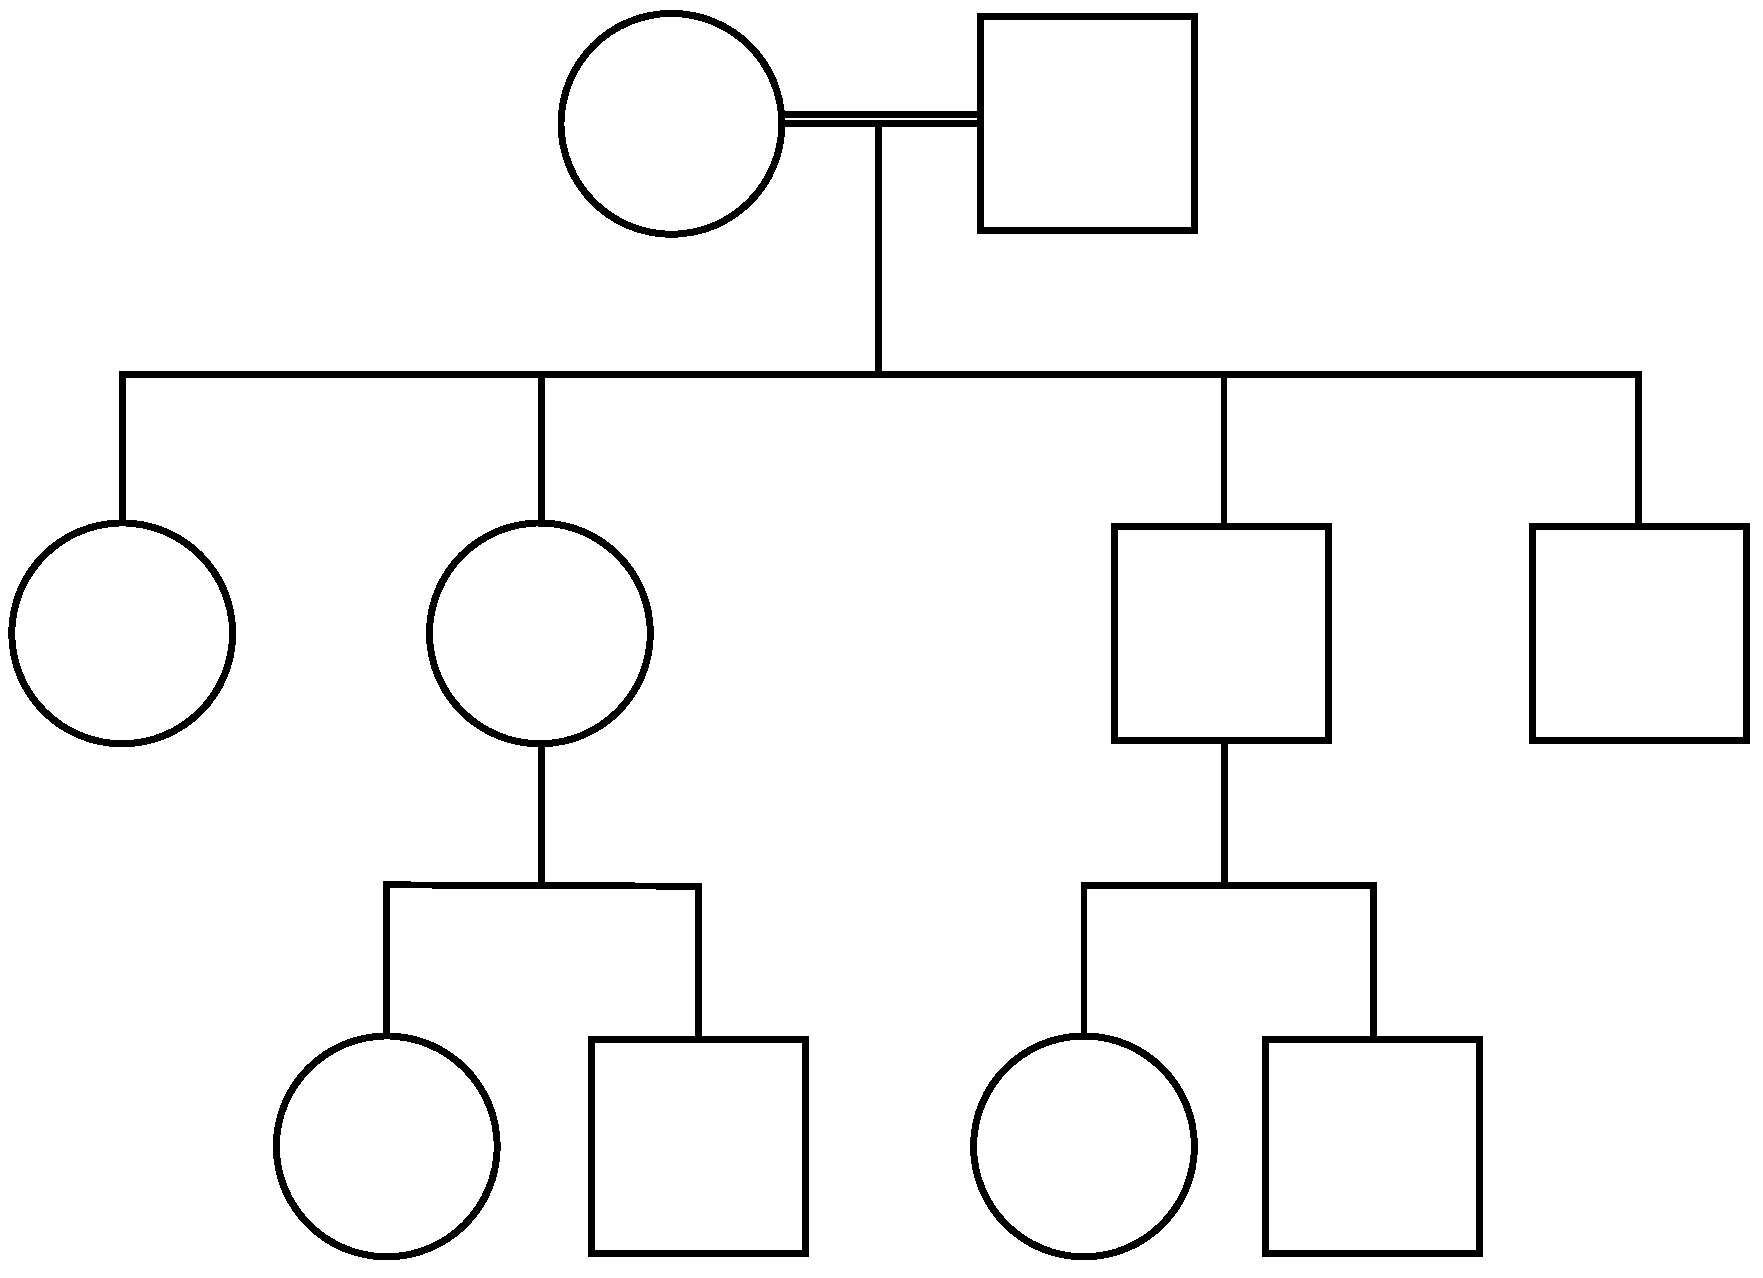
\includegraphics[width = 7cm]{figures/Tabaq.pdf}
\end{figure}

Shortly after, Dr. Hateword had to give up on his research, leaving all his scribbles as well as the blank diagram to his colleague. At first, Dr. Lovelang had no clue as to how he could fill in the diagram, but, after a closer look at the information in the notebook, he managed to fill it in.

Here are the scribbles from the notebook:
\begin{multicols}{2}
\begin{description}[font=\normalfont,leftmargin=!,labelwidth={\widthof{Nadwah:}}]
    \item[Rowa:] \cmubdata{ít̪\`{ɛ} t̪\'{ɛ}\`{ɛ}r} \\ \cmubdata{Minni, t̪\`{ɔ}\`{ɔ}d̪\`{ʊ}} \\ \cmubdata{Nadwah, ít̪\`{ɛ}-n-t̪\`{ɔ}\`{ɔ}d̪\`{ʊ}-t̪\'{ɛ}\`{ɛ}r}
    
    \item[Kuwa:] \cmubdata{Salva, \'{ʊ}t̪\'{ɛ}-k\`{ɔ}t̪\`{ʊ}} \\ \cmubdata{Abdalla, t̪\`{ɔ}\`{ɔ}d̪\`{ʊ}} \\ \cmubdata{Rowa, t̪\`{ɔ}\`{ɔ}d̪\`{ʊ}-t̪\'{ɛ}\`{ɛ}r}
    
    \item[Salva:] \cmubdata{Abir, w\'{ɔ}\'{ɔ}} \\ \cmubdata{Malak, áɲá-n-t̪\`{ɔ}\`{ɔ}d̪\`{ʊ}} \\ \cmubdata{Nadwah, ít̪\`{ɛ} t̪\'{ɛ}\`{ɛ}r}
    
    \item[Sihan:] \cmubdata{Sadiq, ít̪\`{ɛ}} \\ \cmubdata{Minni, ít̪\`{ɛ}-n-t̪\`{ɔ}\`{ɔ}d̪\`{ʊ}-k\`{ɔ}t̪\`{ʊ}} \\ \cmubdata{Kuwa, áfá}
    
    \item[Malak:] \cmubdata{Minni, ít̪\`{ɛ}} \\ \cmubdata{Sihan, màà} \\ \cmubdata{Abdalla, t̪íì}
    
    \item[Sadiq:] \cmubdata{Salva, t̪\`{ɔ}\`{ɔ}d̪\`{ʊ}} \\ \cmubdata{Abir, màà} \\ \cmubdata{Sihan, ít̪\`{ɛ} t̪\'{ɛ}\`{ɛ}r}
    
    \item[Minni:] \cmubdata{Rowa, màà} \\ \cmubdata{Sadiq, t̪íì} \\ \cmubdata{Abir, w\'{ɔ}\'{ɔ}}
    
    \item[Nadwah:] \cmubdata{Kuwa, w\'{ɔ}\'{ɔ}} \\ \cmubdata{Abdalla, fáàfá} \\ \cmubdata{Rowa, áɲá}
    
    \item[Abir:] \cmubdata{Malak, \'{ʊ}t̪\'{ɛ}} \\ \cmubdata{Nadwah, \'{ʊ}t̪\'{ɛ}} \\ \cmubdata{Sadiq, t̪\`{ɔ}\`{ɔ}\textsubbridge{d}\`{ʊ}-k\`{ɔ}t̪\`{ʊ}}
    
    \item[Abdalla:] \cmubdata{Kuwa, áfá} \\ \cmubdata{Malak, ít̪\`{ɛ}-n-t̪\`{ɔ}\`{ɔ}d̪\`{ʊ}} \\ \cmubdata{Salva, ít̪\`{ɛ}-n-t̪\`{ɔ}\`{ɔ}\textsubbridge{d}\`{ʊ}-k\`{ɔ}t̪\`{ʊ}}
\end{description}
\end{multicols}

While filling in the diagram, Dr. Lovelang noticed that, in Tabaq, certain kinship terms can be expressed using two different terms, and one of them is derived from the other. Moreover, he noticed somewhere in the notebook the following information: \textit{Sadiq is a man.} and \textit{Rowa has children.}

\begin{assgts}
\multicolsep=3pt\largerpage[2.5]
\item Fill in the diagram above with the names of the ten family members (in the diagram above circles represents women and squares men). 
\item Write in Tabaq all the possible kinship terms that denote the relation between the following persons:

\begin{multicols}{2}\raggedcolumns
\begin{enumerate}[label = \alph*.]
    \item Sadiq to Salva 
    \item Abir to Nadwah
    \item Salva to Sihan
    \item Nadwah to Minni\columnbreak
    \item Malak to Kuwa
    \item Abdalla to Rowa
    \item Abdalla to Salva
\end{enumerate}
\end{multicols}

\end{assgts}
\end{problem}

\begin{problem}{\langnameAralle}{\nameKGilyarova}{\LOYear{\IOLAbbr}{2016}}
A linguist came to Salu Leang (Sulawesi) to study the Aralle-Tabulahan language. He visited various hamlets of Salu Leang (see the map below) and asked local residents: \cmubdata{Umba laungngola?} \texttr{Where are you going?}

\begin{figure}[H]
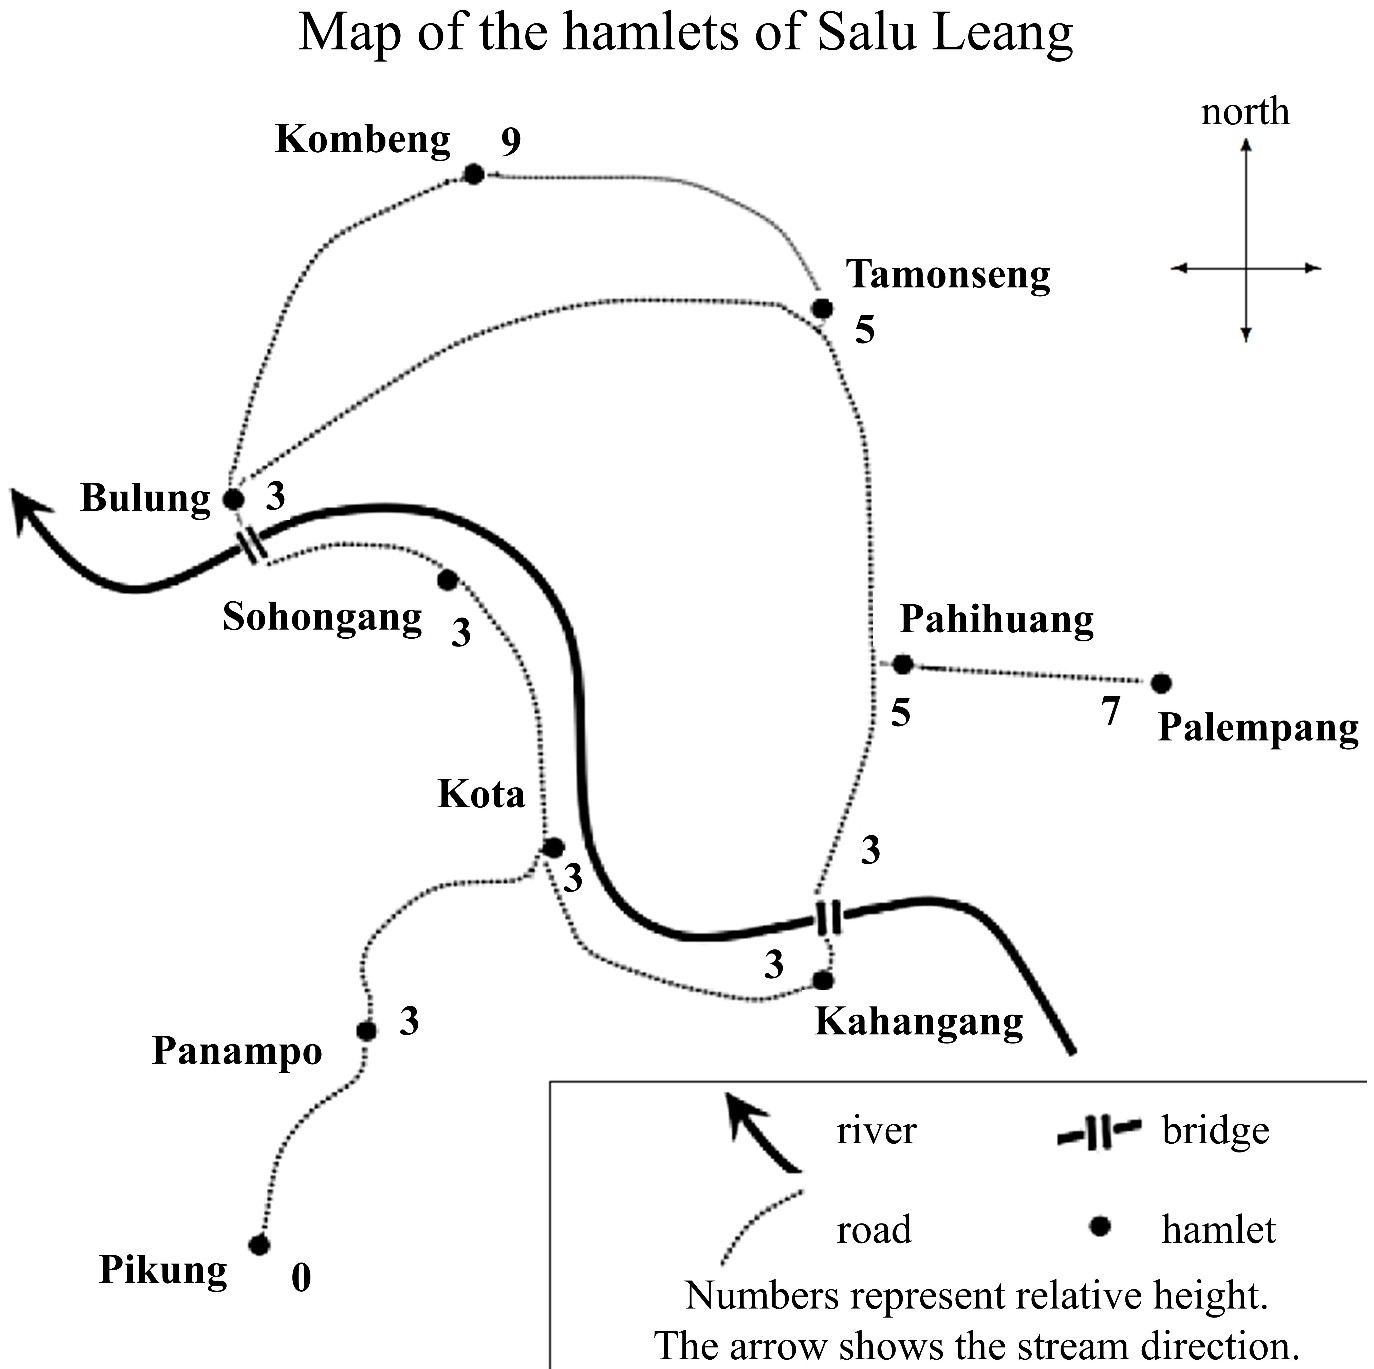
\includegraphics[width=0.75\linewidth]{images/Aralle_EN.jpg}
\end{figure}

Below are the answers he got. There are gaps in some of them.

% % \begin{multicols}{2}
\begin{itemize}[noitemsep]
    \item In {Kahangang} hamlet:
    \begin{itemize}
    \item \cmubdata{Lamaoä' bete' di Bulung.}
    \item \cmubdata{Lamaoä' sau di Kota.}
    \item \cmubdata{Lamaoä' \pbblank di Palempang.}
    \end{itemize}
    \item In {Kombeng} hamlet:
    \begin{itemize}
    \item \cmubdata{Lamaoä' pano di Pahihuang.}
    \item \cmubdata{Lamaoä' tama di Sohongang.}
    \item \cmubdata{Lamaoä' naung di Tamonseng.}
    \item \cmubdata{Lamaoä' \pbblank di Palempang.}
    \end{itemize}
    \item In {Kota} hamlet:
    \begin{itemize}
    \item \cmubdata{Lamaoä' dai' di Kombeng.}
    \item \cmubdata{Lamaoä' dai' di Palempang.}
    \item \cmubdata{Lamaoä' naung di Pikung.}
    \item \cmubdata{Lamaoä' \pbblank di Bulung.}
    \item \cmubdata{Lamaoä' \pbblank di Sohongang.}
    \end{itemize}
    \item In {Palempang} hamlet:
    \begin{itemize}
    \item \cmubdata{Lamaoä' bete' di Kahangang.}
    \item \cmubdata{Lamaoä' dai' di Kombeng.}
    \item \cmubdata{Lamaoä' pano di Panampo.}
    \item \cmubdata{Lamaoä' sau di Sohongang.}
    \item \cmubdata{Lamaoä' \pbblank di Bulung.}
    \item \cmubdata{Lamaoä' \pbblank di Kota.}
    \item \cmubdata{Lamaoä' \pbblank di Pahihuang.}
    \end{itemize}
    \item In {Pahihuang} hamlet:
    \begin{itemize}
    \item \cmubdata{Lamaoä' naung di Bulung.}
    \item \cmubdata{Lamaoä' naung di Pikung.}
    \end{itemize}
    \item In {Bulung} hamlet:
    \begin{itemize}
    \item \cmubdata{Lamaoä' pano di Pahihuang.}
    \item \cmubdata{Lamaoä' pano di Panampo.}
    \item \cmubdata{Lamaoä' \pbblank di Kota.}
    \item \cmubdata{Lamaoä' \pbblank di Pikung.}
    \end{itemize}
    \item In {Panampo} hamlet:
    \begin{itemize}
    \item \cmubdata{Lamaoä' tama di Kahangang.}
    \item \cmubdata{Lamaoä' pano di Tamonseng.}
    \item \cmubdata{Lamaoä' \pbblank di Kota.}
    \end{itemize}
    \item In {Pikung} hamlet:
    \begin{itemize}
    \item \cmubdata{Lamaoä' pano di Kota.}
    \item \cmubdata{Lamaoä' dai' di Pahihuang.}
    \item \cmubdata{Lamaoä' sau di Sohongang.}
    \item \cmubdata{Lamaoä' \pbblank di Bulung.}
    \item \cmubdata{Lamaoä' \pbblank di Kahangang.}
    \item \cmubdata{Lamaoä' \pbblank di Panampo.}
    \end{itemize}
    \item In {Sohongang} hamlet:
    \begin{itemize}
    \item \cmubdata{Lamaoä' bete' di Bulung.}
    \item \cmubdata{Lamaoä' tama di Kahangang.}
    \item \cmubdata{Lamaoä' tama di Kota.}
    \item \cmubdata{Lamaoä' dai' di Pahihuang.}
    \end{itemize}
    \item In {Tamonseng} hamlet:
    \begin{itemize}
    \item \cmubdata{Lamaoä' pano di Pahihuang.}
    \item \cmubdata{Lamaoä' pano di Panampo}
    \item \cmubdata{Lamaoä' \pbblank di Kahangang.}
    \item \cmubdata{Lamaoä' \pbblank di Palempang.}
    \end{itemize}
\end{itemize}
% % \end{multicols}
\begin{assgts}
\item \fillblanks
\end{assgts}
\end{problem}

\begin{problem}{\langnameAkan}{\nameKGilyarova}{\LOYear{\IOLAbbr}{2018}}
Below three Akan men who belong to one family introduce themselves and some members of their family (see the family tree): 
\begin{enumerate}
    \item \cmubdata{Yɛfrɛ me Enu. Yɛfrɛ me banom Thema ne Yaw ne Ama. Yɛfrɛ me yere Kunto. Yɛfrɛ me nuanom Awotwi ne Nsia. Yɛfrɛ me wɔfaase Berko.}
    \item \cmubdata{Yɛfrɛ me Kofi. Yɛfrɛ me nua Esi. Yɛfrɛ me agya Ofori. Yɛfrɛ me se\-waa\-nom Dubaku ne Kunto. Yɛfrɛ me sewaabanom Yaw ne Ama ne Kobina.}
    \item \cmubdata{Yɛfrɛ me Kobina. Yɛfrɛ me ɛnanom Dubaku ne Kunto. Yɛfrɛ me nuanom Yaw ne Ama. Yɛfrɛ me wɔfa Ofori. Yɛfrɛ me yere Efua.}
\end{enumerate}

\begin{figure}[H]
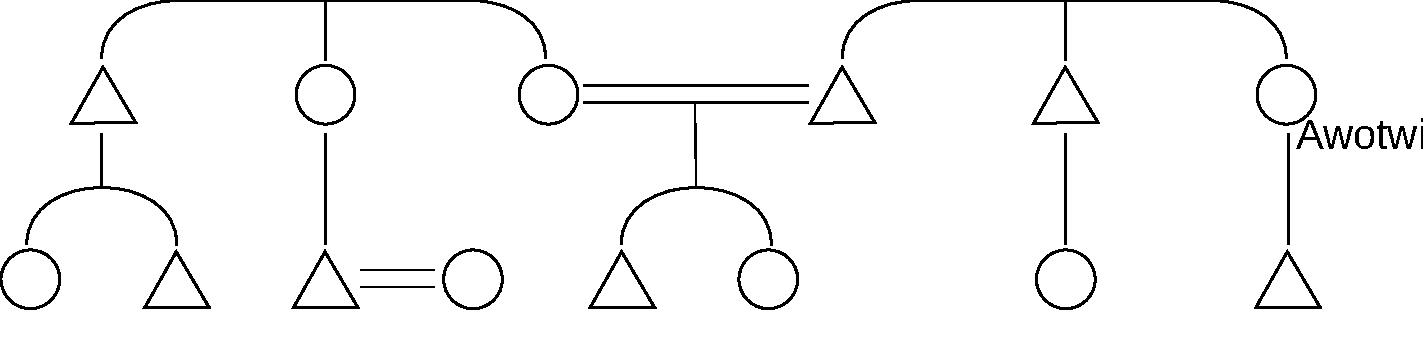
\includegraphics[width = \textwidth]{figures/akan.pdf}\smallskip\\
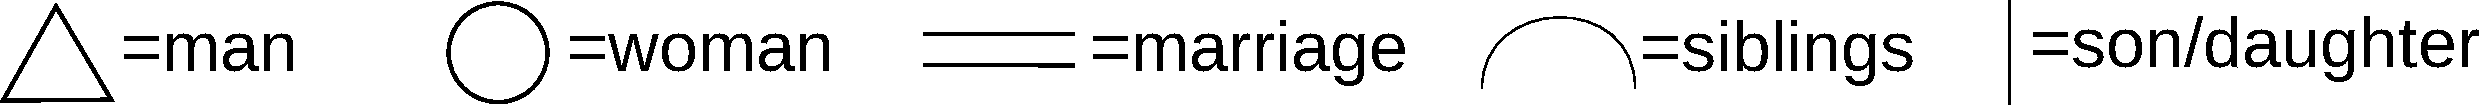
\includegraphics[width = 0.8\textwidth]{figures/akan_legend.pdf}
\end{figure}

\begin{assgts}
\item Supply the family tree with names.
\item Here are some more statements by two other men from this family:
\begin{enumerate}[start = 4]\sloppy
    \item \cmubdata{Yɛfrɛ me Yaw. Yɛfrɛ me ɛnanom \pbblank. Yɛfrɛ me \pbblank Nsia ne \pbblank. Yɛfrɛ me nuanom Thema ne \pbblank. Yɛfrɛ me \pbblank A\-wot\-wi. Yɛfrɛ me \pbblank Ofori. Yɛfrɛ me \pbblank Esi ne \pbblank. Yɛ\-frɛ me \pbblank Berko.}
    \item \cmubdata{Yɛfrɛ me \pbblank. Yɛfrɛ me banom Kofi ne \pbblank. Yɛ\-frɛ me\\ \pbblank \-Yaw ne \pbblank. Yɛfrɛ me \pbblank Kunto ne \pbblank.}
\end{enumerate}
\item[] Fill in the gaps. Some gaps contain more than one word.
\end{assgts}
\end{problem}

\hypertarget{solutions-of-practice-problems}{%
\section{Solutions of practice problems}}

\begin{practiceproblemsolution}{10.3. \langnameBardi}

\begin{solutions}[label=Solution 10.3\alph*]
    \item 1-l, 2-g, 3-k, 4-b, 5-j, 6-f, 7-i, 8-a, 9-d, 10-m, 11-c, 12-h, 13-e.
\end{solutions}
\end{practiceproblemsolution}


\begin{practiceproblemsolution}{10.4. \langnameKharia}

\begin{solutions}[label=Solution 10.4\alph*]
    \item
    \begin{multicols}{3}
        \begin{enumerate}[label = \alph*.]
            \item Dele
            \item Kepka
            \item Mariya
            \item Anil
            \item Beni
            \item Thuyu
            \item Rut
            \item Olem
            \item Muni
            \item Ewa
            \item Sim
            \item Nuh
            \item Kolo
        \end{enumerate}
    \end{multicols}
    \item
    \begin{multicols}{2}
        \begin{enumerate}
            \item \cmubdata{Sowiɲaʔ}
            \item \cmubdata{Dad=iɲaʔ}
            \item \cmubdata{Kolo oɖoyoʔ no Olem}
            \item \cmubdata{Beni}
            \item \cmubdata{Apaiɲaʔ}
            \item[]
        \end{enumerate}
    \end{multicols}
    \item
        \begin{multicols}{3}
        \begin{enumerate}[start = 6]
            \item \cmubdata{Bhaiiɲaʔ}
            \item \cmubdata{Be\textsuperscript{ʔ}ʈiɲaʔ}
            \item \cmubdata{Didikiiɲaʔ}
        \end{enumerate}
    \end{multicols}
\end{solutions}

\rules

Sentence structure: [Kinship term]--(\textsc{pl})--\cmubdata{iɲaʔ} \cmubdata{ɲimi}--(\textsc{pl}) [Persons]
\begin{enumerate}
        \item \textsc{pl} = \cmubdata{-ki-} = plural marker (if there is more than one person)
        \item Persons: Their names; if it's more than one person, \wordtrans{oɖoyoʔ no}{and} is added before the last one.
        \item Kinship terms:

        \begin{multicols}{2}
            \begin{itemize}
                \item \wordtrans{bhai}{younger brother}
                \item \wordtrans{dad=}{older brother} (plural: \cmubdata{dadaki})
                \item \wordtrans{konon bahin}{younger sister}
                \item \wordtrans{didi}{older sister}
                \item \wordtrans{be\textsuperscript{ʔ}ʈ}{son}
                \item \wordtrans{apa}{father}
                \item \wordtrans{sow}{husband}
                \item \wordtrans{đonkui}{brother's wife}
            \end{itemize}
        \end{multicols}
\end{enumerate}

\end{practiceproblemsolution}


\begin{practiceproblemsolution}{10.5. \langnameEmbaloh}

\begin{solutions}[label=Solution 10.5\alph*]
    \item On the first day, when he was told the four directions, he automatically assumed that they represented cardinal directions. In reality, they are based on the topography of the area and represent the relative positions with respect to the river. As such:
        \begin{itemize}
            \item[] \wordtrans{andoor}{towards (closer to) the river}
            \item[] \wordtrans{anait}{away from the river}
            \item[] \wordtrans{urait}{upstream}
            \item[] \wordtrans{kalaut}{downstream}
            \item[] \wordtrans{suali}{across the river}
        \end{itemize}
    \item
    \begin{multicols}{3}
        \begin{enumerate}
            \item \cmubdata{kalaut}
            \item \cmubdata{andoor}
            \item \cmubdata{suali}
        \end{enumerate}
    \end{multicols}
\end{solutions}
\end{practiceproblemsolution}



\begin{practiceproblemsolution}{10.6. \langnameHungarian}

\begin{center}
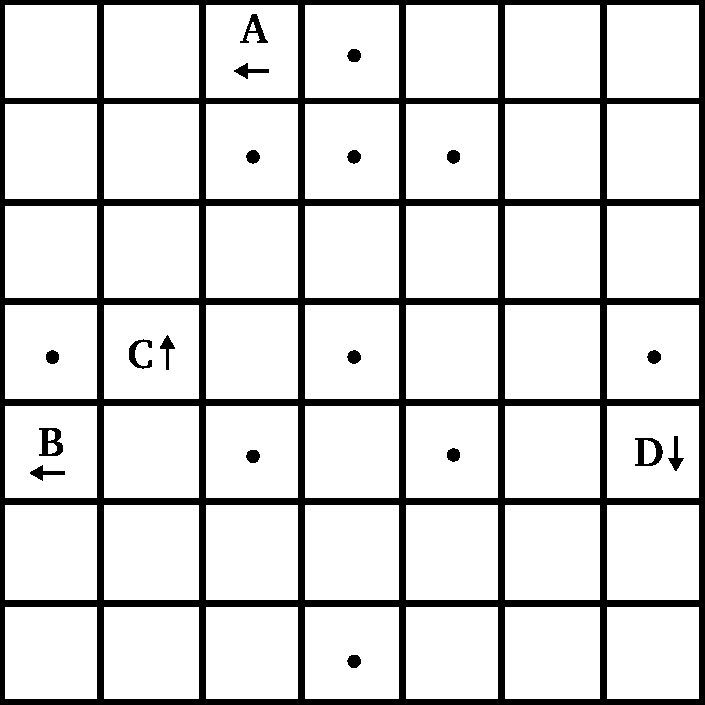
\includegraphics[width = 8 cm]{figures/Hungarian_Squares_solution.pdf}
\end{center}
\begin{multicols}{3}
\begin{itemize}[noitemsep]
    \item[] \wordtrans{előttem}{front}
    \item[] \wordtrans{mögöttem}{back}
    \item[] \wordtrans{balra}{left}
    \item[] \wordtrans{jobbra}{right}
    \item[] \wordtrans{északra}{north}
    \item[] \wordtrans{délre}{south}
    \item[] \wordtrans{nyugatra}{west}
    \item[] \wordtrans{keletere}{east}
    \item[] \wordtrans{nincs}{0}
    \item[] \wordtrans{egy}{1}
    \item[] \wordtrans{két}{2}
    \item[] \quad
\end{itemize}
\end{multicols}
\end{practiceproblemsolution}



\begin{practiceproblemsolution}{10.7. \langnameTabaq}

\begin{solutions}[label=Solution 10.7\alph*]
    \item The names in the diagram are, from left to right:

    \begin{itemize}
        \item[] Top generation: Abir, Kuwa
        \item[] Middle generation: Sihan, Rowa, Sadiq, Abdalla
        \item[] Bottom generation: Malak, Minni, Nadwah, Salva
    \end{itemize}
    \item
    \begin{enumerate}[label = \alph*.]

        \item \cmubdata{áfá}
        \item \cmubdata{wɔ́ɔ́}
        \item \cmubdata{ít̪ɛ̀-n-t̪ɔ̀ɔ̀d̪ʊ̀} or \cmubdata{ít̪ɛ̀-n-t̪ɔ̀ɔ̀d̪ʊ̀-kɔ̀t̪ʊ̀}
        \item \cmubdata{tíì-n-t̪ɔ̀ɔ̀d̪ʊ̀} or \cmubdata{tíì-n-t̪ɔ̀ɔ̀d̪ʊ̀-t̪ɛ́ɛ̀r}
        \item \cmubdata{ʊ́t̪ɛ́} or \cmubdata{ʊ́t̪ɛ́-t̪ɛ́ɛ̀r}
        \item \cmubdata{ít̪ɛ̀} or \cmubdata{ít̪ɛ̀-kɔ̀t̪ʊ̀}
        \item \cmubdata{fáàfá}
    \end{enumerate}
\end{solutions}

\rules

The kinship terms are:
\begin{multicols}{2}
    \begin{itemize}
        \item[] \cmubdata{ít̪ɛ̀}* = \texttr{sibling}
        \item[] \cmubdata{t̪ɔ̀ɔ̀d̪ʊ}* = \texttr{child}
        \item[] \cmubdata{ʊ́t̪ɛ́}* = \texttr{grandchild}
        \item[] \cmubdata{ít̪ɛ̀-n-t̪ɔ̀ɔ̀d̪ʊ̀}* = \texttr{nephew, niece}
        \item[] \wordtrans{wɔ́ɔ́}{grandparent}
        \item[] \wordtrans{áɲá}{father's sister}
        \item[] \wordtrans{màà}{mother, mother's sister}
        \item[] \wordtrans{fáàfá}{father's brother}
        \item[] \wordtrans{tíì}{mother's brother}
        \item[] \wordtrans{áfá}{father}
    \end{itemize}
\end{multicols}

The words marked with * can receive the suffixes \cmubdata{-t̪ɛ́ɛ̀r} and \cmubdata{-kɔ̀t̪ʊ̀}, in order to mark the gender (feminine and masculine, respectively).

The structure \cmubdata{X-n-t̪ɔ̀ɔ̀d̪ʊ} is translated as \texttr{X's child} (thus, a nephew/niece is actually translated as the \texttr{child of the sibling}). The words \cmubdata{màà}, \cmubdata{áɲá}, \cmubdata{tíì}, and \cmubdata{fáàfá} can be combined with \cmubdata{-n-t̪ɔ̀ɔ̀d̪ʊ̀} to express \texttr{cousin}.\\

\end{practiceproblemsolution}


\begin{practiceproblemsolution}{10.8. \langnameAralle}

\begin{solutions}[label=Solution 10.8\alph*]
    \item
    \begin{multicols}{4}
        \begin{enumerate}

            \item \cmubdata{dai'}
            \item \cmubdata{dai'}
            \item \cmubdata{bete'}
            \item \cmubdata{sau}
            \item \cmubdata{naung}
            \item \cmubdata{sau}
            \item \cmubdata{naung}
            \item \cmubdata{tama}
            \item \cmubdata{naung}
            \item \cmubdata{pano}
            \item \cmubdata{bete'}
            \item \cmubdata{tama}
            \item \cmubdata{dai'}
            \item \cmubdata{bete'}
            \item \cmubdata{dai'}
            \item[] \quad
        \end{enumerate}
    \end{multicols}
\end{solutions}

\rules

Basic directions are:
\begin{multicols}{2}
    \begin{itemize}

        \item[] \wordtrans{bete'}{across the river}
        \item[] \wordtrans{tama}{upstream}
        \item[] \wordtrans{sau}{downstream}
        \item[] \wordtrans{pano}{on a flat road}
        \item[] \wordtrans{dai'}{upwards}
        \item[] \wordtrans{naung}{downwards}
    \end{itemize}
\end{multicols}

\end{practiceproblemsolution}


\begin{practiceproblemsolution}{10.9. \langnameAkan}

\begin{solutions}[label=Solution 10.9\alph*]
    \item \quad

    \noindent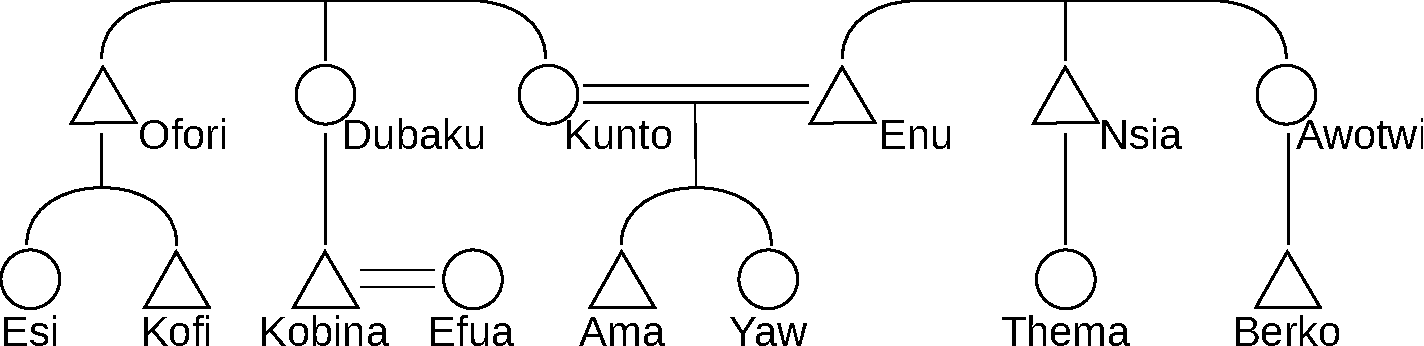
\includegraphics[width = \linewidth]{figures/akan_solutions.pdf}
    \item
    \begin{multicols}{2}
        \begin{enumerate}[leftmargin = 2em, label = (\arabic*)]
            \item \cmubdata{Dubaku ne Kunto}
            \item \cmubdata{agyanom}
            \item \cmubdata{Enu}
            \item \cmubdata{Ama ne Kobina}
            \item \cmubdata{sewaa}
            \item \cmubdata{wɔfa}
            \item \cmubdata{wɔfabanom}
            \item \cmubdata{Kofi}
            \item \cmubdata{sewaaba}
            \item \cmubdata{Ofori}
            \item \cmubdata{Esi}
            \item \cmubdata{wɔfaasenom}
            \item \cmubdata{Ama ne Kobina}
            \item \cmubdata{nuanom}
            \item \cmubdata{Dubako}
        \end{enumerate}
    \end{multicols}
\end{solutions}

\rules
\begin{itemize}
    \item \wordtrans{Yɛfrɛ me N.}{My name is N.}
    \item \wordtrans{Yɛfrɛ me R N.}{My R's name is N.} (\cmubdata{R} = kinship term)
    \item \wordtrans{X ne Y}{X and Y}
    \item \cmubdata{-nom} = \textsc{pl}
    \item Kinship terms:
    \begin{multicols}{2}
    \begin{itemize}
        \raggedright
        \item \wordtrans{ɛna}{mother, mother's sister}
        \item \wordtrans{wɔfaase}{sister's child}
        \item \wordtrans{sewaa}{father's sister}
        \item \wordtrans{sewaaba}{father's sister's child}
        \item \wordtrans{nua}{sibling, parallel cousin}
        \item \wordtrans{agya}{father, father's brother}
        \item \wordtrans{ba}{child, brother's child}
        \item \wordtrans{wɔfa}{mother's brother}
        \item \wordtrans{wɔfaba}{mother's brother's child}
        \item \wordtrans{yere}{wife}
    \end{itemize}
    \end{multicols}
\end{itemize}
\end{practiceproblemsolution}

% \section{Further reading}
% \begin{enumerate}[{label=[\arabic{*}]}]
%     \item Dousset, Laurent. “Australian aboriginal kinship: an introductory handbook with particular emphasis on the Western Desert.”\ \textit{Pacific-Credo Publications}, Marseilles (2012).
%     \item Fortescue, Michael. “Orientation systems of the North Pacific Rim.”\ \textit{The University of Chicago Press}, Chicago (2011).
%     \item Levinson, Stephen C. “Space in language and cognition: explorations in cognitive diversity.”\ \textit{Cambridge University Press}, Cambridge (2003).
%     \item Parkin, Robert. “How Kinship Systems Change.”\ \textit{Berghahn Books}, New York (2021).
% \end{enumerate}
\nocite{Dousset2012, Fortescue2011, Levinson2003, Parkin2021}
% \printbibliography[heading=FurtherReading]
\FurtherReadingBox{}
\end{refsection}
